% !TeX document-id = {88ddee8b-8eb6-46e0-9af4-2c10d8b61c04}
% !TeX spellcheck = de-DE
% !TeX encoding = utf8
% !TeX TXS-program:compile = txs:///pdflatex/[--shell-escape]

% This is LLNCS.DEM the demonstration file of
% the LaTeX macro package from Springer-Verlag
\documentclass[a4paper,12pt]{llncs}
%
\usepackage{makeidx}  % allows for indexgeneration
\makeindex

\usepackage[ngerman]{babel}
\usepackage[utf8]{inputenc}      % Code-Page latin 1
\usepackage[T1]{fontenc}
% Nur eine der beiden folgenden Zeilen einbinden!
% siehe Abschnitt Bilder
\usepackage{graphicx}       % Bilder einbinden, Version fuer normales latex
%\usepackage[pdftex]{graphicx}       % Bilder einbinden, Version fuer pdflatex

% mit Hyperrefs
\usepackage[pdftex, plainpages=false,hypertexnames=true,pdfnewwindow=true,backref=true,colorlinks=true,citecolor=blue,linkcolor=black,urlcolor=blue,filecolor=blue]{hyperref}% 
% weitere Packages
\usepackage{ifthen}                 % Zum Auskommentieren von Textteilen
\usepackage{amssymb}                % Mathematische Buchstaben
\usepackage{amsmath}                % Verbesserter Formelsatz
%\usepackage[vlined,boxed]{algorithm2e}
\usepackage{booktabs}               % schönere Tabellen
\usepackage{color}
\usepackage{algpseudocode}			% Für Pseudocode Algorithmen
\usepackage{tcolorbox}
\usepackage{hyperref}
 \hypersetup{urlcolor=black,citecolor=black}

%\setalcapskip{1.5ex} % fuer package algorithm
\usepackage{dsfont}  
%\newtheorem{definition}{Definition}
\usepackage{doc}
\usepackage{mathrsfs}
\usepackage{mathtools}
\usepackage{todonotes}
\usepackage{subfigure}
\usepackage{pdflscape}
\usepackage{pdfpages}

% Seitenformat ===============================================================
\hoffset=-1.25truecm
\setlength{\topmargin}{0.0cm}
\setlength{\textheight}{23.0cm}
\setlength{\footskip}{1.5cm}
\setlength{\textwidth}{15.4cm}
\setlength{\evensidemargin}{1.5cm}
\setlength{\oddsidemargin}{1.5cm}
\setlength{\parskip}{1ex}
\setlength{\parindent}{0pt}
\setlength{\marginparwidth}{1.4cm}
\setlength{\marginparsep}{1mm}

\pagestyle{plain}

% Makro-Definitionen ==========================================================

% 
\def\myverzeichnis{.}

\numberwithin{equation}{section} 
% Bild -----------------------------------------------------------------------
% #1 Filename;  #2 Label;  #3 Bildunterschrift;  #4 Kurzform
\newcommand{\bild}[4]{
  \begin{figure}[htbp]
    \begin{center}
      \includegraphics{#1}
      \caption[#4]{#3}
      \label{#2}
    \end{center}
  \end{figure}
}

% Bildbreite -----------------------------------------------------------------
% #1 Filename;  #2 Breite;  #3 Label;  #4 Bildunterschrift;  #5 Kurzform
\newcommand{\bildbreite}[5]{
  \begin{figure}[htbp]
    \begin{center}
      \includegraphics[width=#2]{#1}
      \caption[#5]{#4}
      \label{#3}
    \end{center}
  \end{figure}
}

\newtheorem{satz}{Satz}
\newtheorem{korollar}{Korollar}

\DeclareMathOperator{\hit}{hit}
\DeclareMathOperator{\shot_count}{shot\_count}
\DeclareMathOperator{\strat}{strat}
\DeclareMathOperator{\strategies}{strategies}


% ============================================================================
\begin{document}

% =========== Das war der Vorspann, jetzt geht's los! ========================

% ============================================================================
% =============  AB HIER DARF UND SOLL GETIPPT WERDEN ========================
% ============================================================================
\author{Joel Bienias, Samuel Bühner, Dennis Kreittner, Christopher Schnickr}
%\index{Viel Schreiber}

% Das Institut wird fuer den Betreuer missbraucht ...
\institute{{\bf Betreuer:} Dirk Pflüger}
%\institute{{\bf Prüfer:} Prof. Dirk Pflüger}
%\authorrunning{Joel Bienias, Samuel Bühner, Dennis Kreittner, Christopher Schnick}
\title{Hochdimensionales Schiffe Versenken \\
(High-Dimensional Battleship)}

\maketitle

\thispagestyle{empty}

\begin{abstract}
Ein schöner Abstract. Das ist einfach die Kurzzusammenfassung.
\end{abstract}

% Einleitung -----------------------------------------------------------------
\section{Einleitung}

\subsection{Spielbeschreibung}
Diese Ausarbeitung beschäftigt sich mit der Umsetzung von Schiffe-Versenken in beliebig viele Dimensionen.
Die generelle Funktionsweise von dem normalen Schiffe-Versenken bleibt erhalten, muss jedoch um folgende Dinge erweitert werden, um auch in höheren Dimensionen gut spielbar zu sein:

...

Zu Beginn werden eine beliebige Anzahl an Schiffen auf dem Spielfeld platziert.
Die Gesamtheit aller gewählten Schiffspositionen wird auch die Flotte genannt.
Es wird davon ausgegangen, dass die Schiffspositionen rein zufällig ausgewählt wurden, d.h. dass zu Spielbeginn eine Flotte aus der Menge aller möglichen Flotten ausgewählt wird. Jede mögliche Flotte hat hierbei die gleiche Wahrscheinlichkeit, ausgewählt zu werden.
Nun kann der Spieler anfangen, auf bestimmte Positionen auf dem Spielfeld, auch Zellen genannt, zu schießen.
Da Schiffe überlappen können, können mit jedem Schuss mehrere Schiffe, also Teilmengen der Flotte getroffen werden.
Nach jedem Schuss erfährt der Spieler, welche Schiffe der Flotte er getroffen hat.
Ein Schiff gilt als versenkt, sobald es getroffen wurde.
Sobald alle Schiffe versenkt wurden, ist das Spiel beendet.
Das Ziel des Spielers ist es, mit möglichst wenig Schüssen alle Schiffe zu versenken.
Diese Spielregeln sind äquivalent zu denen in \cite{}.


\subsection{Inhalt}

Zum Anfang werden die in der Spielbeschreibung genannten Konzepte mit einigen Definitionen formalisiert, damit sie später angewendet werden können.

Der zweite Teil dieser Ausarbeitung beschäftigt sich dann mit der Bewertung einer gegebenen Strategie, d.h. mit der Berechnung der Anzahl an Schüssen, die mit einer Strategie für verschiedene Flotten benötigt werden.
Da diese Berechnung sehr aufwändig ist, wird ein Monte-Carlo Algorithmus zur Berechnung beschrieben und implementiert.

Im dritten Teil werden unter den zuvor etablierten Rahmenbedingungen verschiedene Strategien vorgestellt und implementiert. Zu den Strategien zählen dünne und volle Gitter, klassisches und Quasi Monte Carlo.

Im letzten Teil werden die Ergebnisse für die genannten Strategien präsentiert, ausgewertet und miteinander verglichen.

\section{Formalisierung des Spielprinzips}

\begin{definition}
Sei
\[
C_{all} \coloneqq \{1, \dots, N\}^d
\]
die Menge aller Zellen des Spielfeldes mit jeweils $N$ Zellen in $d$ Dimensionen.
\end{definition}

\begin{satz}
Dann gilt:
\[
|C_{all}|=N^d
\]
\end{satz}

\begin{definition}
Seien $c, c' \in C_{all}$ Zellen.
Dann ist
\[
c \leq c' \Leftrightarrow \forall i \in \{1, \dots, d\} \colon c_{i} \leq c'_{i} 
\]
\end{definition}

\begin{definition}
Sei $c_{min} \in C_{all}$ und $c_{max} \in C_{all}$ mit $c_{min} \leq c_{max}$.
\[
l=(c_{min}, c_{max})
\]
eine mögliche Schiffsposition (location), welche mithilfe einer minimalen Ecke $c_{min}$ und einer maximalen Ecke $c_{max}$ bestimmt wird.
\end{definition}

\begin{definition}
Sei 
\[
L_{all} \coloneqq
\{
(i, j) \in C_{all} \times C_{all}
\mid
i \leq j
\}
\] die Menge aller möglichen Schiffspositionen.
\end{definition}

\begin{satz}
Dann gilt:
\[
|L_{all}|=\left(\frac{(N+1) N}{2}\right)^d
\]
\end{satz}

\begin{proof}
Da das Spielfeld in jeder Dimension die Größe $N$ hat, gilt in jeder Dimension $d$ für gültige Start- und Endkoordinaten eines Schiffes $c_d$ und $c'_d$ mit $c_d \leq c'_d$ folgendes:
\begin{align}
\begin{split}
&|\{(c_d, c'_d) \in N \times N \mid c_d \leq c'_d\}|\\
&=|\{(i, j) \in N \times N \mid i \leq j\}|\\
&=\sum_{i=1}^N N - i + 1\\
&=N + \sum_{i=1}^{N-1} i\\
&=\sum_{i=1}^{N} i\\
&= \frac{(N + 1) N}{2}
\nonumber
\end{split}
\end{align}
Daher gibt es genau
\[
\left(\frac{(N+1) N}{2}\right)^d
\]
gültige Schiffspositionen, da für jede Schiffsposition für jede Dimension gültige Start- und Endkoordinaten gewählt werden müssen, also genau $d$ gültige Start- und Endkoordinaten.
\end{proof}

\begin{definition}
Sei 
\[
K \coloneqq \{1, \dots, |L_{all}|\}
\]
die Menge aller möglichen Flottengrößen.
\end{definition}

\begin{definition}
Sei $k \in K$ die Größe der Flotte.
Dann ist
\[
F_{all,k} \coloneqq\{F \in \mathcal{P}(L_{all}) \mid |F| = k\}
\]
die Menge aller Flotten der Größe $k$.
\end{definition}

\begin{satz}
Sei $k \in K$ die Größe der Flotte.
Dann gilt:
\[
|F_{all,k}|=\binom{|L_{all}|}{k}
\]
\end{satz}

\begin{definition}
Dann ist
\[
F_{all} \coloneqq \bigcup_{k=1}^{|L_{all}|} F_{all,k} = \mathcal{P}(L_{all}) \setminus \{\emptyset\}
\]
\end{definition}

\begin{definition}
Sei $L \subseteq L_{all}$.
Dann ist
\[
F(L) \coloneqq \mathcal{P}(L) \setminus \{\emptyset\}
\]
die Menge aller Flotten, die mit Schiffen aus $L$ gebildet werden können.
\end{definition}

\begin{satz}
Sei $L \subseteq L_{all}$.
Dann gilt:
\[
|F(L)|=2^{|L|} - 1
\]
\end{satz}

\begin{proof}
\begin{align}
\begin{split}
&|F(L)|=|\mathcal{P}(L) \setminus \{\emptyset\}|=|\mathcal{P}(L)|-1=2^{|L|} - 1
\end{split}
\end{align}
\qed
\end{proof}

\begin{satz}
Dann gilt außerdem:
\[
|F_{all}|=2^{|L_{all}|} - 1
\]
\end{satz}

\begin{proof}
\begin{align}
\begin{split}
&|F_{all}|=\sum_{k=1}^{|L_{all}|} |F_{all,k}|\\
=&\sum_{k=1}^{|L_{all}|} \binom{|L_{all}|}{k} \\
=&\left( \sum_{k=0}^{|L_{all}|} \binom{|L_{all}|}{k} \right) - 1 \\
=&2^{|L_{all}|} - 1
\end{split}
\end{align}
\qed
\end{proof}

\subsection{Strategien}

\begin{definition}
Eine Funktion der Form
\begin{align}
&\strat:\{1,\dots,|C_{all}|\} \rightarrow C_{all} \nonumber
\end{align}
wird Strategiefunktion genannt. Diese wählt die nächste Zelle aus, auf die geschossen werden soll, abhängig davon, auf wieviele Zellen bereits geschossen wurden.
\end{definition}

\begin{definition}
Sei
\[
\strategies  \coloneqq \{ \strat:\{1,\dots,|C_{all}|\} \rightarrow C_{all} \}
\]
die Menge an allen Strategiefunktionen.
\end{definition}

\begin{definition}
Sei $F \in F_{all}$ und $c \in C_{all}$.
Dann ist 
\begin{align}
&\hit:F_{all} \times C_{all} \rightarrow \mathcal{P}(L_{all}) \quad mit \nonumber\\
&\hit(F, c)\mapsto \{(c_{min}, c_{max}) \in F \mid c_{min} \leq c \leq c_{max}\} \nonumber
\end{align}
die Treffer-Funktion, welche angibt, welche Schiffe bei einem Schuss auf Zelle $c$ getroffen wurden, falls $F$ die platzierte Flotte ist. In anderen Worten, die Menge der Schiffe aus Flotte $F$, die die Zelle $c$ belegen.
\end{definition}

\begin{definition}
Sei $F\in F_{all}$ die gewählte Flotte.
Sei außerdem $\strat \in \strategies$ die verwendete Schuss-Strategie.
Dann ist
\begin{align}
&\shot_count(F, \strat)=\min_n \left( \bigcup_{i=1}^n \{hit(F, \strat(i))\} = F \right)
\nonumber
\end{align}
die Anzahl an Schüssen, die benötigt werden, um alle Schiffe der Flotte $F$ mit der Schuss-Strategiefunktion $\strat$ zu versenken.
\end{definition}

\subsection{Schiffe}

\begin{definition}
Sei $\Omega_L \subseteq L_{all}$ eine Menge an Schiffen.
\end{definition}

\begin{definition}
Sei $\omega \in \Omega_L $ das Ereignis, dass das Schiff $\omega$ aus $\Omega_L $ ausgewählt wird.
Dann ist
\[
P(\omega) = \frac{1}{|\Omega_L|}
\]
die Wahrscheinlichkeit, dass das Schiff $\omega$ ausgewählt wird.
\end{definition}

Dann ist $(\Omega_L, P)$ ein endlicher Laplacescher W-Raum und P eine Gleichverteilung.

\begin{definition}
Sei $\strat \in \strategies$ die verwendete Schuss-Strategie.
Sei $\Omega_L \subseteq L_{all}$ eine Menge an Schiffen.
Sei $\omega \in \Omega_L$.
Dann ist
\begin{align}
\mathbf{T}^{\Omega_L}_{\strat}(\omega) = \shot_count(\omega, \strat)
\nonumber
\end{align}
eine Zufallsvariable, die die Anzahl an Schüssen zum versenken eines Schiffes $\omega$ aus $\Omega_L$ bezeichnet.
\end{definition}

\subsection{Flotten}

\begin{definition}
Sei $\Omega_F \subseteq F_{all}$ eine Menge an Flotten.
\end{definition}

\begin{definition}
Sei $\omega \in \Omega_F$ das Ereignis, dass die Flotte $\omega$ aus $\Omega_F$ ausgewählt wird.
Dann ist
\[
P(\omega) = \frac{1}{|\Omega_F|}
\]
die Wahrscheinlichkeit, dass die Flotte $\omega$ ausgewählt wird.
\end{definition}

Dann ist $(\Omega_F, P)$ ein endlicher Laplacescher W-Raum und P eine Gleichverteilung.

\begin{definition}
Sei $\strat \in \strategies$ die verwendete Schuss-Strategie.
Sei $\Omega_F \subseteq F_{all}$ eine Menge an Flotten.
Sei $\omega$ die ausgewählte Flotte aus $\Omega_F$.
Dann ist
\begin{align}
\mathbf{X}^{\Omega_F}_{\strat}(\omega) = \max_{l \in \omega} \shot_count(l, \strat)
\nonumber
\end{align}
eine Zufallsvariable, die die Anzahl an Schüssen zum versenken einer Flotte $\omega$ aus $\Omega_F$ bezeichnet.
\end{definition}

\section{Berechnung des Erwartungswertes mithilfe eines MC-Algorithmus}

Um zu bewerten, wie gut eine Strategiefunktion $\strat$ abschneidet, kann ein Monte-Carlo Algorithmus implementiert werden. Dafür gibt es gute und weniger gute Ansätze:

\subsection{Der naive Ansatz}

Um zu berechnen, wann eine gegebene Flotte $F$ versenkt wird, kann folgende Funktion verwendet werden:

\begin{tcolorbox}
	\begin{algorithmic}[H]
		\Function{shot\_count}{$F, \strat$}{:}
		\State $S=\emptyset$;
		\State $\shot_count=0$;
		\While{$S \neq F$}
		\State $next\_target=\strat(\shot_count)$;
		\State $S=S \cup \hit(F, next\_target)$;
		\State $\shot_count=\shot_count+1$;
		\EndWhile
		\State\Return $\shot_count$;
		\EndFunction
	\end{algorithmic}
\end{tcolorbox}

Mithilfe dieser Funktion werden dann Werte für $n$ zufällig gewählte Flotten zu einem Erwartungswert der Stichprobe kombiniert:

\begin{tcolorbox}
	\begin{algorithmic}[H]
		\Function{evaluate\_strategy}{$n, \strat$}{:}
		\State //Generiere $n$ verschiedene Flotten;
		\State $fleets = generate\_random\_fleets(n)$;
		\For{$i=1,\dots,n$}
		\State $shots= shot\_count(fleets[i], \strat)$;
		\State $P(\mathbf{X}^F_{\strat} = shots)+=\frac{1}{n}$;
		\EndFor
		\EndFunction
	\end{algorithmic}
\end{tcolorbox}

Das Problem dieses Ansatzes ist, dass eine zufällig ausgewählte Flotte ziemlich viel Schiffe enthält. Da für jedes Schiff in dieser Flotte irgendwie ermittelt werden muss, wann es versenkt wird, können nur sehr wenige Flotten als Stichprobe benutzt werden, da die Berechnungszeit für eine einzige Flotte schon sehr groß ist.


\subsection{Eine bessere Alternative}

\begin{satz}
Sei $\strat \in \strategies$ die verwendete Schuss-Strategie und $v \in \{1, \dots, |C_{all}|\}$.

Sei $\Omega_L \subseteq L_{all}$ eine Menge an Schiffen und $n=|\Omega_L|$.

Sei $L=\{x \in \Omega_L \mid \shot_count(l, \strat) \leq v)\}$ die Menge an Schiffen aus $\Omega_L$, die nach maximal $v$ Schüssen versenkt werden und $l=|L|$.

Dann ist
\begin{align}
P(\mathbf{T}^{\Omega_L}_{\strat} \leq v) = \frac{l}{n}
\nonumber
\end{align}
die Wahrscheinlichkeit, dass ein Schiff, das zufällig aus $\Omega_L$ ausgewählt wurde, nach maximal $v$ Schüssen versenkt wird.
\end{satz}

\begin{proof}
Es gibt $l$ Schiffe, die nach maximal $v$ Schüssen versenkt werden.

Die Wahrscheinlichkeit, ein Schiff auszuwählen, dass in $L$ liegt, beträgt $\frac{l}{n}$, da es eine Gleichverteilung ist.
\qed
\end{proof}

Bestimmt man nun $P(\mathbf{T}^{\Omega_L}_{\strat} \leq v)$ mithilfe einer so groß wie möglichen Stichprobe $\Omega_L$, kann man annehmen, dass $P(\mathbf{T}^{\Omega_L}_{\strat} \leq v)$ eine Approximation von $P(\mathbf{T}^{L_{all}}_{\strat} \leq v)$ ist. Wie gut diese Approximation ist, hängt von der Stichprobengröße ab.

Um nun die Verteilungsfunktion von Flotten zu bestimmen, wird im folgenden wird nun davon ausgegangen, dass gilt:
\[
P(\mathbf{T}^{\Omega_L}_{\strat} \leq v) \approx P(\mathbf{T}^{L_{all}}_{\strat} \leq v)
\]
d.h. unsere aus der Stichprobe berechnete Verteilungsfunktion ist die beste Approximation von der echten Verteilungsfunktion.

Ein Sampling error $e_v=P(\mathbf{T}^{\Omega_L}_{\strat} \leq v) - P(\mathbf{T}^{L_{all}}_{\strat} \leq v)$ verstärkt sich zwar bei der Berechnung von der Verteilungsfunktion der Flotten um ca. den Faktor $2^{e_v |L_{all}|} - 1$, wie aber gleich zu sehen ist, macht dies bei den sehr kleinen Werten von $P(\mathbf{X}^{F_{all}}_{\strat} \leq v)$ fast keinen Unterschied.

\begin{satz}
Sei $\strat \in \strategies$ die verwendete Schuss-Strategie und $v \in \{1, \dots, |C_{all}|\}$
Sei außerdem $l=P(\mathbf{T}^{L_{all}}_{\strat} \leq v) |L_{all}|$

Dann ist
\begin{align}
P(\mathbf{X}^{F_{all}}_{\strat} \leq v) = \frac{2^{l} - 1}{2^{|L_{all}|} - 1} \approx 2^{l - |L_{all}|}
\nonumber
\end{align}
die Wahrscheinlichkeit, dass eine Flotte, die zufällig aus $F_{all}$ ausgewählt wurde, nach maximal $v$ Schüssen versenkt wird.
\end{satz}

\begin{proof}
Sei $L=\{x \in L_{all} \mid \shot_count(l, \strat) \leq v)\}$ die Menge an Schiffen aus $L_{all}$, die nach maximal $v$ Schüssen versenkt werden.
Dann ist $F(L)$ die Menge an Flotten aus $F_{all}$, die nach maximal $v$ Schüssen versenkt werden.

Außerdem gilt $|L|=l=l \frac{|L_{all}|}{|L_{all}|}=P(\mathbf{T}^{L_{all}}_{\strat} \leq v) |L_{all}|$ und daher gibt es $|F(L)|=2^l - 1$ Flotten in $F_{all}$, die nach maximal $v$ Schüssen versenkt werden.

Die Wahrscheinlichkeit, eine Flotte aus $F_{all}$ auszuwählen, die in $F(L)$ liegt, beträgt $\frac{2^l - 1}{2^n - 1}$, da es eine Gleichverteilung ist.
\qed
\end{proof}

Die Folge dieser Verteilungsfunktion für Flotten ist, dass die Werte sehr klein sind.

\begin{definition}
Eine Funktion der Form
\begin{align}
&I_{\strat}:C_{all} \rightarrow \{1, \dots, |C_{all}|\} = \strat^{-1} \nonumber
\end{align}
wird Indexfunktion einer Strategie genannt. Diese weißt jeder Zelle des Spielfeldes den Wert zu, zu welchem die Zelle getroffen wird.
\end{definition}

Der Vorteil der Indexfunktion ist, dass diese Werte einmalig für eine Strategie berechnet werden müssen und dann in einem Array abgespeichert werden können. Dafür müssen dann Zellen in einen Array-Index umgewandelt werden können.

Damit kann man eine Alternative Definition von $\mathbf{T}^{\Omega_L}_{\strat}$ angeben:

\begin{definition}
Sei $\strat \in \strategies$ die verwendete Schuss-Strategie.
Sei $\Omega_L \subseteq L_{all}$ eine Menge an Schiffen.
Sei $\omega \in \Omega_L$.
Dann ist
\begin{align}
\mathbf{T}^{\Omega_L}_{\strat}(\omega) = \min_{c \in cells(\omega)} I_{\strat}(c)
\nonumber
\end{align}
eine Zufallsvariable, die die Anzahl an Schüssen zum versenken eines Schiffes $\omega$ aus $\Omega_L$ bezeichnet.
\end{definition}


In folgendem effizienteren Algorithmus werden die gespeicherten Werte der Indexfunktion $I_{\strat}$ verwendet, um zu ermitteln, nach wie vielen Schüssen ein Schiff versenkt wird. 

\begin{tcolorbox}
	\begin{algorithmic}[H]
		\Function{calculate\_turns}{$n, \strat$}{:}
		\State //Generiere $n$ verschiedene Schiffe;
		\State $\Omega_L = generate\_random\_ships(n)$;
		\State $turns = [1, ..., |C_{all}|]$;
		\State $sum=0$;
		\For{$i=1,\dots,n$}
		\State $min= \min_{c \in cells(\Omega_L[i])} I_{\strat}(c)$;
		\State $turns[min]++$;
		\EndFor
		\State\Return $turns$;
		\EndFunction
	\end{algorithmic}
\end{tcolorbox}

Es wird aus den Ergebnissen von einer Stichprobe mit $n$ Schiffen $\Omega_L$ die Verteilungsfunktion $P(\mathbf{T}^{\Omega_L}_{\strat} \leq v)$ bestimmt. Unter der Annahme, dass $P(\mathbf{T}^{\Omega_L}_{\strat} \leq v) \approx P(\mathbf{T}^{L_{all}}_{\strat} \leq v)$ gilt, wird damit dann die Verteilungsfunktion für Flotten, $P(\mathbf{X}^{F_{all}}_{\strat} \leq v)$ bestimmt:

\begin{tcolorbox}
	\begin{algorithmic}[H]
		\Function{evaluate\_strategy}{$n, \strat$}{:}
		\State $turns = calculate\_turns(n, \strat)$;
		\State $ship\_sum=0$;
		\For{$i=1,\dots,|C_{all}|$}
		\State $ships=turns[i]$;
		\State $ship\_sum += ships$;
		\State $P(\mathbf{T}^{\Omega_L}_{\strat} \leq i)=\frac{ship\_sum}{n}$;
		\State $P(\mathbf{X}^{F_{all}}_{\strat} \leq i)=\frac{2^{\left(P(\mathbf{T}^{\Omega_L}_{\strat} \leq i) * |L_{all}|\right)} - 1}{2^{|L_{all}|} - 1}$;
		\EndFor
		\EndFunction
	\end{algorithmic}
\end{tcolorbox}

\section{Strategien}


Eine Strategie gibt eine Folge von Schüssen vor, die auf das Spielfeld abgegeben werden. Dabei unterscheiden sich die Strategien in der Auswahl ihrer Schüsse. Eine mögliche Vorgehensweise wäre die zufällige Wahl der nächsten zu beschießenden Zelle. Im Vergleich dazu ist es interessant zu sehen wie diskrepanzminimierende Diskretisierungsverfahren als mögliche Schussstrategie abschneiden. Dies wurde erstmals in \cite{M13} näher betrachtet. Dabei werden die von diesen Verfahren genutzten Stützstellen als Schussfolgen interpretiert. Um Strategien bewerten zu können benötigt man den Vergleich zu einer optimalen Schussstrategie. Diese wurde ebenfalls in \cite{M13} vorgestellt allerdings für ineffizient erklärt. Es bleibt zu klären, ob die optimale Strategie mit der hier vorgestellten Monte-Carlo Herangehensweise effizienter umzusetzen ist und zu Vergleichen auch in höheren Dimensionen herangezogen werden kann.


\subsection{Maximum Strategie oder optimale Strategie}

Diese in \cite{M13} Abbildung 3.15 vorgestellte Strategie ist optimal, da sie immer an die Position schießt an der sie zu jedem Zeitpunkt am meisten Schiffe auf einmal treffen und damit versenken kann. Dazu wird zunächst eine Anfangsverteilung berechnet. Jeder Zelle wird die Anzahl der darauf liegenden Schiffe zugewiesen. Der nächste Schuss wird auf die Zelle mit der größten Zahl abgegeben. Schließlich wird die Verteilung aktualisiert um die gerade versenkten Schiffe.

Die optimale Strategie kann durch folgenden Algorithmus in Pseudo-Code beschrieben werden:

\begin{tcolorbox}
	\begin{algorithmic}
		\Function{max\_strat}{$S$}{$:\text{cell}$}
		\State $\text{cell} = null$;
		\State $\text{max} = 0$;
		\State $\text{temp} = 0$;
		\For{\textbf{each } $c\in C_{all}$}
		\State $\text{temp}=\left|\hit(F,c)\right|$;
		\If{$\text{temp}>\text{max}$}
		\State $\text{max}=\text{temp}$;
		\State $\text{cell} = c$;
		\EndIf
		\EndFor
		\State \Return $\text{cell}$;
		\EndFunction
	\end{algorithmic}
\end{tcolorbox}

In \cite{M13} wurde bereits angesprochen, dass dieser Algorithmus sehr hohe Kosten hat. Obiger Code wird über alle Zellen des Spielfelds iteriert, das heißt wir haben $N^d$ Schleifendurchläufe pro Aufruf der Strategie. In jedem dieser Durchläufe wird die $\hit$ Funktion aufgerufen. Diese muss für jedes Schiff aus der aktuellen Flotte $F$ prüfen ob dieses die momentan anvisierte Zelle $c$ enthält. Diese Überprüfung kann mittels zwei arithmetischen Vergleichen (Erinnerung: ein Schiff wird als Tupel $(c_{min},c_{max})$ gespeichert) erledigt werden. Damit haben wir für den Aufruf der $\hit$ Funktion Kosten von $O(2\cdot |F|)$, bzw. $O(F)$. Somit betragen sich die gesamten Kosten der optimalen Strategie auf $O(N^d\cdot F)$.
 

\subsection{Volle Gitter Strategie}

\subsubsection{Allgemeines zu Gittern}

In Abschnitt 2.2.1 von \cite{M13} werden die hierarchischen Stützstelleninkremente $H_{\underline{m}}$ für Gitter vorgestellt, welche sich von den in \cite{M13} Abbildung 2.2 dargestellten Hütchenfunktionen ableiten. Diese Inkremente bzw. ihre Kombinationen werden sowohl für dünne als auch volle Gitter genutzt. Dabei halbiert sich die Maschenweite mit steigendem Koordinatenlevel in einer beliebigen Dimension. Dies ist schön zu sehen in Abbildung \ref{fig:gitter01} (ähnlich aufgebaut wie \cite{P10} Figure 2.5).

Es lassen sich durch Kombinationen von Inkrementen Gitter erzeugen. Unsere Schussfolge ergibt sich dann aus den abgearbeiteten Inkrementen bzw. den darin enthaltenen Stützstellen. 

\begin{figure}
	\centering
	\resizebox{90mm}{!}{\input{figures/Grids_01.pdf_tex}}
	\caption{Verdeutlichung Halbierung der Maschenweite}
	\label{fig:gitter01}
\end{figure}


Noch zu beachten ist, dass Koordinatenlevel bei Gittern die Maschenweite und damit die Genauigkeit angeben. Normalerweise legt man ein Gitterlevel fest und erzeugt sich dann aus Inkrementen ein Gitter eben dieses Levels. In unseren Fall arbeiten wir uns durch die Inkremente bei steigendem Gitterlevel aufsteigend durch um immer genauere Gitter zu erzeugen, bis wir alle Schiffe der Flotte getroffen haben.

\subsubsection{Mathematische Grundlagen der vollen Gitter}

In \cite{M13} Definition 2.14 wird beschrieben, wie sich volle Gitter aus den Inkrementen zusammensetzen. Dabei ist lediglich zu beachten, dass die Indices eines Inkrements $H_{\underline{m}}$ nur kleiner dem Gitterlevel $n$ sein müssen.  Zur Wiederholung:

\begin{definition}
	Seien $d,n\in\mathbb{N}$ und $d,n>1$. Ein $d$-dimensionales volles Gitter $G$ mit Gitterlevel $n$ wird durch Kombination der Inkremente $H_{\underline{m}}$ mit $\underline{m}<(n,\dots,n)$ erzeugt:
	\begin{equation}
		G=\biguplus_{m_1=1}^n\biguplus_{m_2=1}^n\dots \biguplus_{m_d=1}^n H_{\underline{m}}
	\end{equation}
\end{definition}

Diese Definition kann anhand Abbildung \ref{fig:gitter02} verdeutlicht werden. Darin sind einige mögliche Kombinationen von Inkrementen markiert, die ein volles Gitter von Gitterlevel 2 bis 4 bilden.

\begin{figure}
	\subfigure[Volles Gitter Gitterlevel 2]{\resizebox{50mm}{!}{\input{figures/Grids_02.pdf_tex}}}
	\subfigure[Volles Gitter Gitterlevel 3]{\resizebox{50mm}{!}{\input{figures/Grids_03.pdf_tex}}}
	\subfigure[Volles Gitter Gitterlevel 4]{\resizebox{50mm}{!}{\input{figures/Grids_04.pdf_tex}}}
	\caption{Inkremente von zweidimensionalen vollen Gittern}
	\label{fig:gitter02}
\end{figure}

Wie man gut an Abbildung \ref{fig:gitter02} sehen kann können volle Gitter kleineren Gitterlevels als Teilbausteine für Größere genutzt werden. Für eine Schussfolge heißt das man startet bei dem Gitter das nur aus einem Punkt besteht und arbeitet sich zu Gittern höheren Gitterlevels vor. Damit bei der Schussfolge keine Wiederholungen auftreten sollten nur neu hinzugekommene Punkte bei Erhöhen des Gitterlevels beachtet werden. Im zweidimensionalen entspricht dies gerade Quadraten die bei Erhöhen des Gitterlevels um eine Längeneinheit pro Kante wachsen. Dabei wird dann lediglich die hinzukommende Schicht an Punkten betrachtet. Damit lässt sich einer Schussfolge bereits eine grobe Struktur geben. 

Außerdem ist an Abbildung \ref{fig:gitter02} zu sehen, dass in den neu hinzukommenden Punkten mindestens eine neue Koordinaten verwendet wird. Das heißt wir können pro neuer Schicht zu Beginn einmalig die neuen Koordinaten berechnen und anschließend diese einfach aufsteigend miteinander zu Punkten kombinieren. Dabei können Schüsse wie Zahlen in einem Zahlensystem betrachtet werden. Wir denken uns die verwendeten Koordinaten aus denen Schüsse kombiniert werden können als Ziffern eines Zahlensystems. Dabei sind Koordinaten eines höheren Koordinatenlevels größer einzuordnen als die eines niedrigeren. Außerdem werden die Koordinaten innerhalb eines Koordinatenlevels von klein nach groß sortiert. Damit ergibt sich eine absolute Ordnung der Punkte und Schüsse dieser Strategie lassen sich durch Hochzählen der Zahlen des Zahlensystems bestimmen.

Von diesen Koordinaten gibt es maximal $N$ viele. Diese werden im nachfolgenden Algorithmus in $K$ gespeichert.

\subsubsection{Erster naiver Algorithmus für volle Gitter Strategie}

Der Algorithmus soll eine feste Menge an möglichen Koordinaten $K$ für ein Koordinatenlevel $L$ als globale Variablen verwenden. Davon werden alle Linearkombinationen durch inkrementieren der Koordinaten (vgl. absolute Ordnung) gebildet. Sobald alle Kombinationen erreicht wurden wird $K$ um die neuen Koordinaten des nächsten Koordinatenlevels erweitert. Außerdem muss der letzte abgegebene Schuss gespeichert werden um daraus den nächsten Schuss zu berechnen. Diese grobe Struktur lässt sich folgendermaßen darstellen:

\begin{tcolorbox}
	\begin{algorithmic}
		\Function{full\_grid\_strat}{}{$:\text{cell}[]$}
		\State $\text{cell}[]\text{ shots} = \text{ new } \text{cell}[C_{all}]$
		\State $\text{lastShot}=null$ ; $\text{lastIndices}=null$
		\State int $L$;
		\For{int $i=0$ ; $i<C_{all}$ ; $i++$}
		\If{$K=\emptyset$}
		\State \textsc{initiate\_Coordinates}()
		\EndIf
		\If{$\text{lastShot}=(\text{max\_coord},\dots,\text{max\_coord})$}
		\State \textsc{add\_New\_Coordinates}()
		\EndIf
		\If{$\text{lastShot} = null$}
		\State $\text{lastIndices} = (0,\dots,0)$
		\State $\text{lastShot} = (K[0],\dots,K[0])$
		\State $\text{shots}[i] = \text{lastShot}$
		\Else
		\State \textsc{increment\_Coordinates}()
		\EndIf
		\EndFor
		\State\Return $\text{shots}$
		\EndFunction
	\end{algorithmic}
\end{tcolorbox}

Die Strategie returniert alle Schüsse auf das gesamte Spielfeld in einem Array. Dabei ist bei Index $i$ im Array der $i+1$ Schuss als Zelle gespeichert.

Im folgenden werden die Abschnitte und Funktionen des Algorithmus genauer betrachtet und ihre Komplexität untersucht.

\begin{tcolorbox}
	\begin{algorithmic}
		\Function{initiate\_Coordinates}{}{}
		\State $K=\left[\left\lfloor\frac{N}{2}\right\rfloor\right]$
		\State $\text{max\_coord}=K\left[0\right]$
		\State $L=0$
		\EndFunction
	\end{algorithmic}
\end{tcolorbox}

Mit dieser Funktion wird die erste Koordinate initialisiert. Wenn $K$ leer haben wir noch keine Koordinate gespeichert und daher auch noch keinen Schuss abgegeben. Die erste Koordinate, die für das erste volle Gitter benutzt wird ist gerade die Größe des Spielfelds $N$ halbiert. Falls $N$ ungerade ist wird abgerundet. max\_coord enthält die maximal mögliche Koordinate. $L$ beschreibt das maximale Koordinatenlevel von dem unsere Koordinaten in $K$ stammen. Gesamte Komplexität $O(1)$.

\smallskip
\hrule
\smallskip
\begin{tcolorbox}
	\begin{algorithmic}
		\Function{add\_New\_Coordinates}{}
		\State $min=\left\lceil\frac{K[2^L-1]}{2}\right\rceil$
		\State $K_{old}=K\left[2^L-1\dots 2^{L+1}-2\right]$
		\For{\textbf{each } $k\in K_{old}$}
		\If{$K[last\_index]!=k-min$}
		\State $K.add(k-min)$
		\EndIf
		\State $K.add(k+min)$
		\EndFor
		\State $L++$
		\State $\text{max\_coor}d=K\left[2^{L+1}-2\right]$
		\EndFunction
	\end{algorithmic}
\end{tcolorbox}

Wenn der letzte Schuss nur aus den größtmöglichen Koordinaten besteht haben wir bereits zuvor alle anderen Kombinationsmöglichkeiten ausgenutzt und müssen nun die Menge an Koordinaten $K$ erweitern. Dazu werden gerade die Werte als Koordinaten hinzugefügt, die in den Zwischenräumen zweier vorheriger Koordinaten liegen (Vgl. Abbildung \ref{fig:gitter01}). 

Da wir in unserer Herangehensweise diskret arbeiten kann es sein, dass das Halbieren nicht immer aufgeht daher muss hier gerundet werden. Es wird aufgerundet, da sonst der Fall eintreten kann, das Punkte nicht erreicht werden können. Dabei wird durch eine Abfrage gewährleistet das keine gleichen Koordinaten aufgenommen werden. Zum Schluss wird die Menge der Koordinaten aktualisiert und das Koordinatenlevel erhöht. $K$ kann maximal um $\left\lceil\frac{N}{2}\right\rceil$ viele neue Koordinaten erweitert werden. Das ist gleichzeitig auch die maximal mögliche Größe von $K_{old}$. Also haben wir für die Schleife $O(N)$. 


Der Vergleich im If benötigt $d$ Schritte daher ist die Komplexität $O\left(N+d\right)$.

\smallskip
\hrule
\smallskip

\begin{tcolorbox}
	\begin{algorithmic}
		\If{$\text{lastShot} = null$}
		\State $\text{lastIndices} = (0,\dots,0)$
		\State $\text{lastShot} = (K[0],\dots,K[0])$
		\State $\text{shots}[i] = \text{lastShot}$
		\Else
		\State $\dots$
		\EndIf
	\end{algorithmic}
\end{tcolorbox}

Hier wird geprüft ob wir uns am Anfang des ersten Gitters befinden und der erste Schuss wird entsprechend in das shots Array eingefügt. Außerdem wird lastIndices initialisiert, das die Indices der verwendeten Koordinaten Speichert. Dies erleichtert uns später das Finden des nächsten Schusses. Komplexität $O(1)$.

\smallskip
\hrule
\smallskip

\begin{tcolorbox}
	\begin{algorithmic}
		\Function{increment\_Coordinates}{}
		\State $s=\text{lastShot}$
		\State $\text{count} =d$
		\While{True}
		\If{$s[\text{count}]=\text{max\_coord}$}
		\State $s[\text{count}]=K[0]$
		\State $\text{lastIndices}[\text{count}]=0$
		\State $\text{count}--$
		\Else
		\State $s[\text{count}] = K[\text{lastIndices}[\text{count}]+1]$
		\State $\text{lastIndices}[\text{count}]++$
		\State\textbf{break}
		\State $\text{shots}[i] = \text{lastShot}$
		\EndIf
		\EndWhile
		\EndFunction
	\end{algorithmic}
\end{tcolorbox}

In diesem Abschnitt wird das Inkrementieren im gedachten Zahlensystem realisiert. Dabei wird von der letzten Ziffer nach vorne gehend geprüft welche davon den aktuell maximal möglichen Wert hat. Diese Ziffern müssen beim Zählen dann zurück auf Null bzw. die kleinste Koordinate $K[0]$ springen. Sobald die erste Ziffer erreicht wird, die nicht den maximal Wert hat kann diese um eins erhöht werden. Die restlichen Ziffern, falls vorhanden, bleiben gleich. 

Die Schleife kann maximal $d$ Schritte durchführen. Es wurde bereits vorher ausgeschlossen, dass $s$ nur aus maximalen Koordinaten bestehen kann, also springen wir auf jeden Fall irgendwann innerhalb der $d$ Schritte in den else Teil. 

Der absolute worst case wäre wenn $d-1$ mal der if Teil und einmal der else Teil aufgerufen werden. Das heißt dieser Abschnitt liegt in $O(d)$.

\subsubsection{Komplexität erste volle Gitter Strategie}

Wir können somit die Laufzeitkomplexitäten der Abschnitte zusammenfassen und erhalten eine gesamte Komplexität für einen Durchlauf des Algorithmus von $O(1)+O(N+d)+O(1)+O(d)=O(N+2d)$. Somit ergibt sich als Komplexität für den kompletten Algorithmus $O(C_{all}\cdot (N+2d))$.


Bezüglich der Speicherplatz Komplexität haben wir für $K$ $O(N)$, da für die Anzahl der Elemente in $K$ gilt:

\begin{equation}
\sum_{j=0}^{\log_2(N)-1}2^j\leq N \in O\left(N\right)
\end{equation}


Im Algorithmus werden alle abgegebenen Schüsse in shots gespeichert. Da dies nach diesem Ansatz $C_{all}$ viele sind ergibt das eine gesamte Speicherplatz Komplexität von $O(N+C_{all})$.

Um die Abhängigkeit der Laufzeitkomplexität von $C_{all}$ kommen wir nicht herum, da jede Zelle mindestens einmal betrachtet werden muss. Allerdings ist die Speicherplatzkomplexität zu vermeidbar wie wir später noch sehen werden. 


\subsection{Dünne Gitter Strategie}

\subsubsection{Mathematische Grundlagen der dünnen Gitter}

In \cite{M13} Definition 2.15 wird beschrieben, wie sich dünne Gitter aus den Inkrementen zusammensetzen. Zur Wiederholung:

\begin{definition}
	Seien $d,n\in\mathbb{N}$ und $d,n>1$. Ein $d$-dimensionales dünnes Gitter $G$ mit Gitterlevel $n$ wird durch Kombination der Inkremente $H_{\underline{m}}$ mit $|\underline{m}|_1\leq n+d-1$ erzeugt:
	\begin{equation}
	G=\biguplus_{|\underline{m}|_1\leq n+d-1}^n H_{\underline{m}}
	\end{equation}
\end{definition}

Wobei für die verwendete Norm gilt (Vgl. \cite{P10} Abschnitt 2.1 Basics):

\begin{definition}
Die  $|\cdot|_1$-Norm ist definiert als:
	\begin{equation}
	|\underline{m}|_1:=\sum_{j=1}^d m_j
	\end{equation}
\end{definition}


Die Definition des dünnen Gitters kann anhand Abbildung \ref{fig:gitter03} verdeutlicht werden. Darin sind einige mögliche Kombinationen von Inkrementen markiert, die ein dünnes Gitter von Gitterlevel 1 bis 3 bilden.

\begin{figure}
	\subfigure[Dünnes Gitter Gitterlevel 1]{\resizebox{50mm}{!}{\input{figures/Grids_02.pdf_tex}}}
	\subfigure[Dünnes Gitter Gitterlevel 2]{\resizebox{50mm}{!}{\input{figures/Grids_05.pdf_tex}}}
	\subfigure[Dünnes Gitter Gitterlevel 3]{\resizebox{50mm}{!}{\input{figures/Grids_06.pdf_tex}}}
	\caption{Beispiele für zweidimensionale dünne Gitter}
	\label{fig:gitter03}
\end{figure}

\subsubsection{Erster naiver Algorithmus für dünne Gitter}

In Abbildung \ref{fig:gitter03} ist zu sehen, dass sich im zweidimensionalen Fall bei steigendem Level der Gitter immer eine Diagonale dazukommt. Für den ersten Algorithmus der dünne Gitter Strategie benötigen wir ein $S'$, das Tupel aus zwei $d$-dimensionalen Vektoren speichert. Der erste um die Zelle zu beschreiben und der zweite um das Koordinatenlevel aus der die korrespondierende Koordinate stammt zu definieren. Das neue $K'$ speichert nun die Koordinaten nach Koordinatenlevels getrennt in verschiedenen Listen oder Arrays und nicht wie $K$ noch alles in einer Liste/Array. $S'$ und $K'$ werden global initialisiert.

Die Funktionsweise des folgenden Algorithmus leitet sich von der mit dünne Gittern einhergehenden Bedingung $|\underline{m}|_1\leq n+d-1$ an die Inkremente ab. Bei konstanter Dimension erhöht sich pro dazukommende Diagonale um das nächste Gitter zu erzeugen jeweils nur $n$ um eins. Das heißt von den Indices der Inkremente kann sich maximal eines auf ein neues Koordinatenlevel erhöhen damit die Bedingung weiterhin erhalten bleibt. Also erarbeiten wir ausgehend von den alten die neuen Schüsse, indem einzelne Koordinaten um ein Koordinatenlevel erhöht werden. Dabei ist zu beachten, dass innerhalb eines neuen Koordinatenlevels es mehrere mögliche Koordinaten gibt. 


\begin{tcolorbox}
	\begin{algorithmic}
		\Function{sparse\_grid\_strat}{}{$:\text{cell}[]$}
		\State int $L$; int countcoord; int position
		\State cell[] shots = new cell[$C_{all}$]
		\For{int $i=0$; $i<C_{all}$; $i++$}
		\If{$K'=\emptyset$}
		\State \textsc{initiate\_Coordinates}()
		\EndIf
		\If{$S'[\text{last\_index}][0]=(K'[0][0],\dots,K'[0][0],\text{max\_coord})$}
		\State \textsc{add\_New\_Coordinates}()
		\EndIf
		\If{$S=\emptyset$}
		\State $S'.add((('K[0][0],\dots,K'[0][0]),(0,\dots,0)))$
		\State $\text{shots}[i] = (K'[0][0],\dots,K'[0][0])$
		\Else
		\State \textsc{find\_Next\_Shot}()
		\EndIf
		\EndFor
		\State \Return $\text{shots}$
		\EndFunction
	\end{algorithmic}
\end{tcolorbox}

Die grobe Struktur des Algorithmus ist analog zu vollen Gittern.

Wir werden jetzt nun den Algorithmus in kleinen Teilen näher betrachten und dabei die Funktionsweise und Komplexität genauer beschreiben.

\smallskip
\hrule
\smallskip

\begin{tcolorbox}
	\begin{algorithmic}
		\Function{initiate\_Coordinates}{}
		\State $K'[0]=\left[\left\lfloor\frac{N}{2}\right\rfloor\right]$
		\State $\text{max\_coord}=K'\left[0\right][0]$
		\State $L=0$
		\State $\text{countCoord} = 0$
		\State $\text{position} = 0$
		\EndFunction
	\end{algorithmic}
\end{tcolorbox}

Sollte $K'$ leer sein werden die erste Koordinate hinzugefügt und ein paar notwendige Variablen initialisiert. Auf die Funktion der Variablen $countCoord$ und $position$ kommen wir noch später genauer zu sprechen. Die Komplexität ist $O(1)$.

\smallskip
\hrule
\smallskip

\begin{tcolorbox}
	\begin{algorithmic}
		\Function{add\_New\_Coordinates}{}
		\State $\text{min}=\left\lceil\frac{K'[L][0]}{2}\right\rceil$
		\State $K'.add([])$
		\For{\textbf{each } $k\in K'[L]$}
		\If{$K'[L+1][\text{last\_index}]!=k-\text{min}$}
		\State $K'[L+1].add(k-\text{min})$
		\EndIf
		\State $K'[L+1].add(k+\text{min})$
		\EndFor
		\State $L++$
		\State $\text{max\_coord}=K'\left[L\right][\text{last\_index}]$
		\State $\text{countCoord} = 0$
		\State $\text{position} = 0$
		\EndFunction
	\end{algorithmic}
\end{tcolorbox}

Dieser Abschnitt beschreibt den Fall, dass neue Koordinaten hinzugefügt werden müssen. Dabei ist die Iteration so aufgebaut, dass der letzte Schuss eines Koordinatensatzes gerade die Form $(K'[0][0],\dots,K'[0][0],max\_coord)$ hat. Da von vorne nach hinten durch die Dimensionen gezählt wird und $max\_coord$ ebenfalls die letzte Koordinate eines Koordinatenlevels ist. Es wird nun wie zuvor bereits erwähnt eine neue Liste/Array erzeugt, die die Koordinaten des neuen Koordinatenlevels enthalten soll. Die Berechnungen unterscheiden sich dabei nicht von denen bei vollen Gittern. Zum Schluss werden noch einmal $countCoord$ und $position$ gesetzt, da diese wie wir noch sehen werden, sich im Laufe verändert haben und nun zurückgesetzt werden müssen.

Der Vergleich im If ist in $O(d)$. Die Schleife hat $\left\lceil\frac{N}{4}\right\rceil$ Durchläufe, da das gerade die Anzahl der Elemente im vorletzten Koordinatenlevel ist. Das letzte Koordinatenlevel taucht als Schleife nicht mehr auf, da bis dahin bereits alle Punkte des Spielfelds beschossen sind. Also ist die Schleife in $O(N)$. Davon ausgehend, dass $last\_index$ in $O(1)$ realisiert werden kann hat dieser Abschnitt eine gesamte Komplexität von $O(N+d)$.

\smallskip
\hrule
\smallskip

\begin{tcolorbox}
	\begin{algorithmic}
		\If{$S=\emptyset$}
		\State $S'.add((('K[0][0],\dots,K'[0][0]),(0,\dots,0)))$
		\State $\text{shots}[i] = (K'[0][0],\dots,K'[0][0])$
		\Else
		\State $\dots$
		\EndIf
	\end{algorithmic}
\end{tcolorbox}

Der If Abschnitt liegt in $O(1)$. 

\smallskip
\hrule
\smallskip

\begin{tcolorbox}
	\begin{algorithmic}
		\Function{find\_Next\_Shot}{}
		\State $\text{out} = S'[0]$
		\If{$\text{countCoord}=0$}
		\State $\text{out}[1][\text{position}]++$
		\EndIf
		\State $\text{out}[0][\text{position}]=K[\text{out}[1][\text{position}]][\text{countCoord}]$
		\State $\text{countCoord}++$
		\If{$\text{countCoord}=K[\text{position}].\text{size}()$}
		\State $\text{countCoord}=0$
		\State $\text{position}++$
		\If{$\text{position}=d$}
		\State $\text{position}=0$
		\State $S'.\text{delete}(0)$
		\EndIf
		\EndIf
		\State $S'.\text{add}(\text{out})$
		\State $\text{shot}s[i] = \text{out}[0]$
		\EndFunction
	\end{algorithmic}
\end{tcolorbox}

Die Funktion aus dem Else Abschnitt hat zunächst ein paar $O(1)$ Zeilen, da es sich nur um Zugriff oder arithmetische Operationen handelt. Die $size()$ Funktion liegt bei maximalem Koordinatenlevel in $O(N)$. Die $delete()$ Funktion ist hier $O(1)$, da das erste Element entfernt wird, was in $O(1)$ geht. Somit hat der Else Teil und damit der gesamte Abschnitt eine Komplexität von $O(N)$.

\subsubsection{Komplexität dünne Gitter Strategie}

Für den gesamten Algorithmus ergibt sich also eine aus den Teilfunktionen berechnete Laufzeitkomplexität von $O((1+N+d+1+N)\cdot C_{all}) = O(C_{all}\cdot(2N+d))$.

Der Speicherbedarf ist für $K'$ analog zu $K$ von den vollen Gittern, also $O(N)$. Was $S'$ anbelangt werden hier mehrere Schüsse gespeichert und auch verwendet. Bildlich im Zweidimensionalen gesprochen wird zu jedem Zeitpunkt eine komplette Diagonale an Inkrementen und deren dazugehörige Schüsse gespeichert. Nach \cite{GG08} ist die Anzahl an Punkten für dünne Gitter gegeben als:

\begin{equation}
\left|\hat{V}_n\right| = \sum_{i=0}^{n-1} 2^i \cdot \binom{d-1+i}{d-1}
\end{equation}

Also haben wir einen Speicherbedarf für eine ''Diagonale'' von $O\left(2^L \cdot \binom{d-1+L}{d-1}\right)$. Wir müssen im worst case mindestens auf ein Koordinatenlevel von $L=\log_2(N)$, da nur so alle Punkte im Raum überhaupt erst getroffen werden können. Das heißt wir haben eine untere Schranke an den Speicherplatz einer ''Diagonalen'' von $\Omega\left(N \cdot \binom{d-1+\log_2(N)}{d-1}\right)$. Wir können aber auch nicht mehr Punkte als im Raum vorhanden sind beschießen. Das heißt die untere Schranke bildet gleichzeitig eine obere Schranke. Zusätzlich wird jeder Schuss in shots gespeichert. Somit erhalten wir eine scharfe Schranke für die gesamte Speicherplatzkomplexität von $\Theta\left(N \cdot \binom{d-1+\log_2(N)}{d-1} + N + C_{all}\right)$.

Wie bereits für die vollen Gitter ist solch eine Speicherplatzausnutzung nicht wünschenswert.


\subsection{Monte-Carlo Strategie}

Ähnlich wie Strategien aus der Diskretisierung durch dünne und volle Gitter gewonnen wurden, kann eine Strategie aus der Monte-Carlo Diskretisierung abgeleitet werden. Dabei stellt die Wahl der Stützstellen, die bei Gittern noch nach Gesetzmäßigkeiten ausgewählt wurden, effektiv die Strategie dar, so dass diese Punkte den Schüssen entsprechen. Da bei Monte-Carlo diese Stützstellen zufällig gewählt werden, tun wir dies auch hier für die Monte-Carlo Strategie. 

Diese Strategie kommt einer realen Strategie am nächsten, da die meisten Spieler nach dem Zufallsprinzip vorgehen. Der Algorithmus ist sehr simpel, da lediglich eine zufällige Zelle als Ziel des Schusses gewählt werden muss.

\begin{tcolorbox}
	\begin{algorithmic}
		\Function{monte\_carlo\_strat}{$S$}{$:cell$}
		\State \Return $randomFrom(C_{all}\backslash S)$
		\EndFunction
	\end{algorithmic}
\end{tcolorbox}

Die zufällige Auswahl von Zellen, die nicht bereits beschossen wurden lässt sich leicht realisieren indem man zum Beispiel zuerst alle Zellen durchzählt, wobei auf die erste als erstes geschossen werden soll und die Zellen dann eine Weile miteinander zufällig tauscht. Damit erreicht man eine zufällige Schussfolge.


\subsection{Sobol Strategie}

\subsection{Halton Strategie}
Die Halton Sequenz ist eine Zahlensequenz, die eine niedrige Diskrepanz besitzt und daher nahezu zufällig erscheint.

\subsubsection{Konstruktion einer eindimensionalen Halton Sequenz}
Die Bestimmung von Halton Punkten basiert auf Primzahlen, die als Basis dienen. Um die $i$-te Zahl der Sequenz zu bestimmen wird zuerst die Basisdarstellung von $i$ bestimmt. Sei für eine Primzahl $p$ $i$ in gegeben in Basisdarstellung mit Koeffizienten $a_j$ mit $j\in{0,\dots,k}$ so, dass gilt:
\begin{equation}
i = a_0p^0+\dots+a_kp^k
\end{equation}
Um die zum Index $i$ gehörige Zahl der Halton Sequenz$ i_{\text{Halton}}$ zu erhalten wird die Basisdarstellung folgendermaßen umgewandelt:
\begin{equation}
i_{\text{Halton}} = a_0p^{-1}+a_1p^{-2} + \dots+a_kp^{-(k+1)}
\end{equation}

\subsubsection{Algorithmus zur Halton Sequenz}
Halton Sequenzen mit beliebiger Basis lassen sich mit folgenden Algorithmus erzeugen. Dabei gibt dieser jeweils nur eine Zahl der Sequenz mit dem Index, der dem Algorithmus übergeben wurde.

\begin{tcolorbox}
	\begin{algorithmic}
		\Function{halton}{$\text{base}, \text{index}$}{$:double$}
		\State $\text{coefficient} = 1$
		\State $ \text{result} = 0$
		\While{$\text{index}>0$}
		\State $\text{coefficient} = \text{coefficient} / \text{base}$
		\State $\text{result} = \text{result} + \text{coefficient} \cdot (\text{index}\mod \text{base})$
		\State $\text{index} = \lfloor \text{index}/\text{base} \rfloor $
		\EndWhile
		\State \Return result
		\EndFunction
	\end{algorithmic}
\end{tcolorbox}

\subsubsection{Erzeugen einer Schussstrategie}
Wir benötigen zuerst die Möglichkeit mehrdimensionale Punkte erzeugen zu können. Mehrdimensionale Halton Sequenzen werden durch das Kombinieren von eindimensionalen Sequenzen erreicht. Dazu werden als Basen teilerfremde Primzahlen gewählt und der jeweils $i$-te generierte Punkt der einzelnen Sequenzen bildet eine Koordinate des $i$-ten Punkts in mehreren Dimensionen. Das heißt aus Sequenzen $\left(\frac{1}{2},\frac{1}{4},\frac{3}{4},\dots\right)$ und $\left(\frac{1}{3},\frac{2}{3},\frac{1}{9},\dots\right)$ ergeben sich zweidimensionale Punkte $\left(\left(\frac{1}{2},\frac{1}{3}\right),\left(\frac{1}{4},\frac{2}{3}\right),\left(\frac{3}{4},\frac{1}{9}\right),\dots\right)$.

Anhand dieses Beispiels haben wir bereits das zweite Problem gesehen. Die Zahlenwerte müssen noch auf die Spielfeldgröße erweitert werden. Dies lässt sich leicht durch einer Multiplikation mit $N$ und runden erledigen. Damit würde sich die Ausgabe des Algorithmus ändern zu $\lfloor result * N \rfloor$.

Ein letztes Problem der Halton Sequenz ist, dass es aufgrund des Rundens zu häufigem Beschießen der gleichen Zellen kommt. Das heißt das ein Durchlauf unter gleichen Rahmenbedingungen, also gleiche Dimension, Spielfeldgröße etc., bei Halton länger dauert als andere Strategien, die jedes Feld definitiv nur einmal beschießen. 
 

\section{Implementierung}

\subsection{Allgemeines zur Implementierung}
Aufgrund von begrenztem Arbeitsspeicher und der großen Anzahl an Zellen in höheren Dimensionen müssen Vorkehrungen getroffen werden um das Programm auch auf weniger leistungsstarken Systemen lauffähig zu machen. Dies konnten wir bereits bei der Analyse der Speicherplatzkomplexität der ersten naiven Algorithmen zu vollen und dünnen Gittern beobachten. 

Die Lösung ist das Spielfeld in Blöcke aufzuteilen, die maximal so groß wie der verfügbare Arbeitsspeicher sind. Danach werden die Blöcke sequentiell abgearbeitet. Ein Aufruf einer Strategie bearbeitet also nur einen Block.

Dies bedeutet für die Strategien, dass diese ihre Angaben wann welche Zelle beschossen wird bezüglich eines Blockes machen müssen. Allerdings ist zu beachten, dass die gesamte Strategie sich weiterhin auf das ganze Spielfeld bezieht. Also wäre es nicht korrekt wenn die Strategien unabhängig auf den einzelnen Blöcken ausgeführt werden. Man muss Angaben zu den Zellen einzelner Blöcke machen können ohne die gesamte Schussfolge der Strategie für das Spielfeld zu speichern, da dies mit begrenztem Speicher nicht immer möglich ist. Daraus entstanden die tatsächlichen Implementierungen der Strategien im Gegensatz zum naiven Ansatz zuvor.

\subsection{Allgemeines zu Gittern}

Unser Ansatz arbeitet mit diskreten Zellen und Spielfeldern. Das bedeutet, dass wir an manchen Stellen besonders vorsichtig sein müssen. Wie zum Beispiel bei Redundanzen in den Koordinatenpunkten. Diese können entstehen wenn die Halbierung der Koordinaten der letzten ($\lceil\log_2(N)\rceil$) Koordinatenlevels nicht aufgeht. Durch anschließendes Runden kann es zu doppelt auftretenden Koordinaten kommen. Diese können sich sowohl in anderen Koordinatenlevels als auch im selben Koordinatenlevel wiederholen. Allerdings treten ''Wiederholer'' nur im letzten ($\lceil\log_2(N)\rceil$) Koordinatenlevels auf. Da vorher die Maschenweite noch nicht eng genug war um Kollisionen hervorzurufen. Das bedeutet es muss beachtet werden, dass die tatsächliche Anzahl an neuen Koordinaten, die im letzten Koordinatenlevels dazukommen, kleiner ist als einfach nur das Doppelte des vorherigen Koordinatenlevels. Dies wiederum beeinflusst die Anzahl der Punkte aller Inkremente in deren Index sich mindestens einmal das maximale Koordinatenlevel befindet. Das Auftreten der Redundanzen hängt einzig von der Spielfeldgröße $N$ ab. Nur wenn $N = 2^k-1$ mit $k\in\mathbb{N}$ treten keine Redundanzen auf.

\begin{figure}
	\centering
	\resizebox{.90\linewidth}{!}{\input{figures/redundancy1.pdf_tex}}
	\caption{Beispiel für Redundanz}
	\label{fig:redundancy}
\end{figure}

In der Implementierung spielt die Redundanz nur in den dünnen Gittern eine Rolle.


\subsection{Volle Gitter Strategie}

Die tatsächliche Implementierung muss weiterhin die grobe Struktur des naiven Algorithmus verfolgen, da alles andere schlichtweg falsch wäre. Um es mit der Terminologie des zweidimensionalen Falles auszudrücken, es müssen weiterhin die Schichten nacheinander abgearbeitet werden (vgl. Abbildung \ref{fig:fullGrid01}).

\begin{figure}
	\subfigure[Schicht Giiterlevel 0]{\resizebox{36mm}{!}{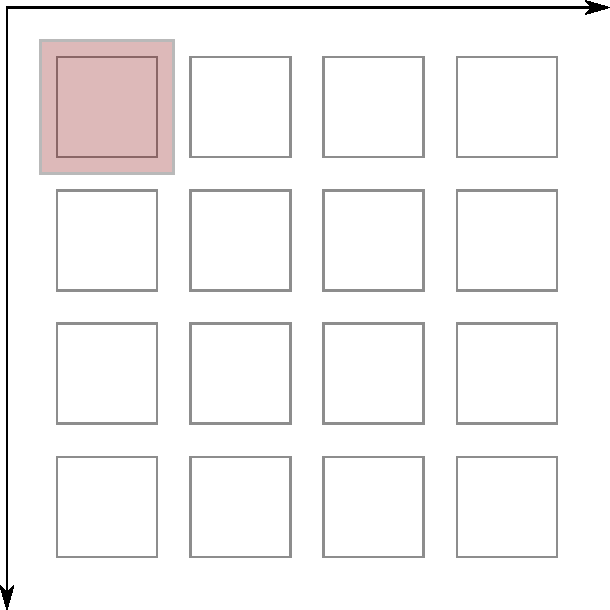
\includegraphics{figures/FullGridGeneral1}}}
	\subfigure[Schicht Giiterlevel 1]{\resizebox{36mm}{!}{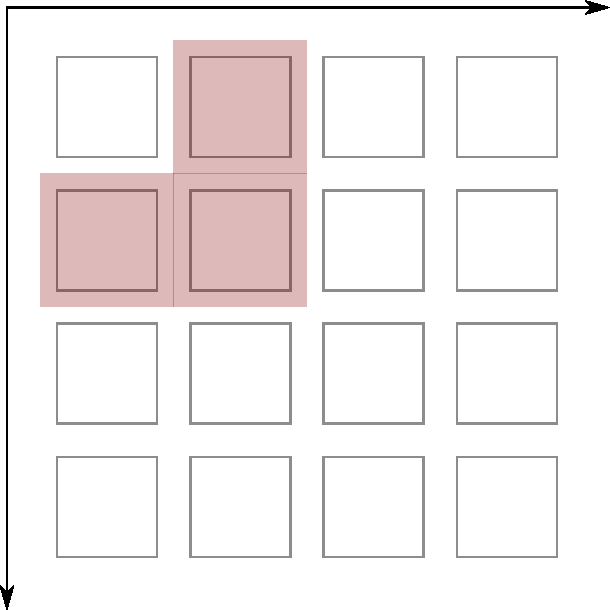
\includegraphics{figures/FullGridGeneral2}}}
	\subfigure[Schicht Giiterlevel 2]{\resizebox{36mm}{!}{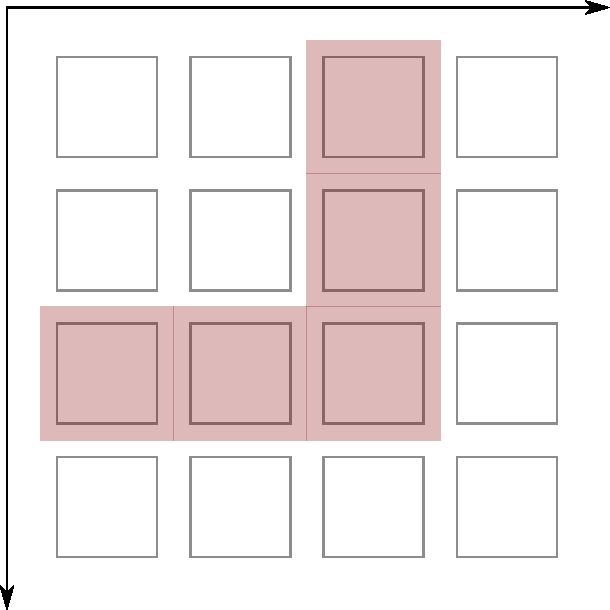
\includegraphics{figures/FullGridGeneral3}}}
	\subfigure[Schicht Giiterlevel 3]{\resizebox{36mm}{!}{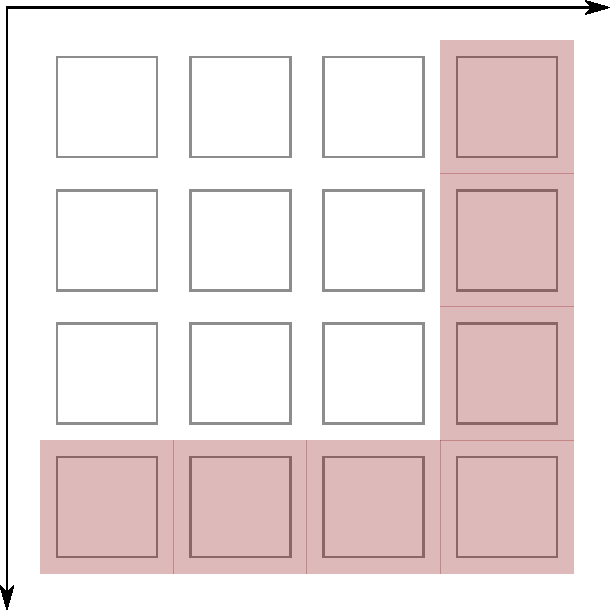
\includegraphics{figures/FullGridGeneral4}}}
	\caption{Grobe Struktur bzgl. Inkremente volle Gitter Strategie 2 Dimensionen}
	\label{fig:fullGrid01}
\end{figure}

\subsubsection{Vorgehen}

Die auf Blöcke abgestimmte volle Gitter Strategie arbeitet relativ simpel. Zunächst wird in MAX\_LEVEL\_FULL[] die maximale Anzahl der pro Gitterlevel neu hinzugekommen Punkte (in 2 Dimensionen also alle Punkte einer Schicht) berechnet und gespeichert . Anschließend wird ein Zähler LEVEL\_FULL[] für jedes Gitterlevel eingerichtet der anfänglich auf 1 steht. Die Strategie iteriert dann über den Block und bestimmt für jeden Punkt in welchem Gitterlevel er liegt. Für dieses Gitterlevel wird dem Punkt dann nur noch der passende Zähler zugewiesen und danach inkrementiert.

\subsubsection{Algorithmus in Pseudocode}

Dem Algorithmus wird eine Referenzkoordinate zum Block und ein Array, das jeder Zelle im Block die Nummer wann sie von der Strategie beschossen wird zuweist, übergeben.

\begin{tcolorbox}
	\begin{algorithmic}
		\Function{fullGridStrat}{int[] blockShots, cell blockCoordinate}{:void}
		\State cell currentCell
		\State int shotNumber
		\For{int $i=0$; $i<$BlockSize; $i++$}
		\State \textsc{getCoordinateFromNumber}()
		\State int max $=0$
		\State max = \textsc{getMaxLevel}()
		\State shotNumber = \textsc{calculateShotnumber}()
		\State blockShot[currentCell] = shotNumber
		\EndFor
		\EndFunction
	\end{algorithmic}
\end{tcolorbox}

\subsubsection{Erläuterung der Funktionen}
Die Funktion \textsc{getCoordinateFromNumber}() berechnet in $O(d)$ Schritten aus $i$ eine Koordinate durch Bestimmung der Koeffizienten der Zahlendarstellung zur Basis $N$. Die ersten Koordinaten werden durch die Blockkoordinaten ergänzt.

Die Funktion \textsc{getMaxLevel}() bestimmt in $O\left(d\cdot 2^{\lceil\log_2(N)\rceil}\right)$ das maximale Gitterlevel von currentCell. Dabei werden alle $d$ Koordinaten der Zelle jeweils mit den $2^{\lceil\log_2(N)\rceil}$ Levelkoordinaten (vgl. Abbildung \ref{fig:redundancy}) verglichen und das maximale Gitterlevel in max gespeichert.

Die Funktion \textsc{calculateShotnumber}() errechnet in $O(max) = O\left(\lceil\log_2(N)\rceil\right)$ Schritten die Schussnummer von currentCell in dieser Strategie. Diese wird bestimmt durch Addition der MAX\_LEVEL\_FULL aller Gitterlevel bis max und LEVEL\_FULL[max]. Schließlich wird noch LEVEL\_FULL[max] inkrementiert.

\subsubsection{Komplexität}
Somit erhalten wir eine Laufzeitkomplexität von \\ $O\left(BlockSize\cdot\left(d\left( 2^{\lceil\log_2(N)\rceil}+1\right)+\lceil\log_2(N)\rceil\right)\right)$ für den vollen Gitter Algorithmus. Die Speicherkomplexität beläuft sich dann auf $O(BlockSize)$. Bei $d$ Dimensionen kann BlockSize variiert werden zwischen $N^1$ und $N^d$. Wobei $N^d$ nur zu empfehlen ist wenn ausreichend Speicher zur Verfügung steht. 

\newpage
\subsection{Dünne Gitter Strategie}

Für die dünnen Gitter gilt das gleiche wie für die vollen, es muss weiterhin die Struktur eingehalten werden. Das heißt in diesem Fall mit der Terminologie für zwei Dimensionen, dass die Diagonalen nacheinander abgearbeitet werden (vgl. Abbildung \ref{fig:sparseGrid01}).

\begin{figure}
	\subfigure[Schicht Level 0]{\resizebox{36mm}{!}{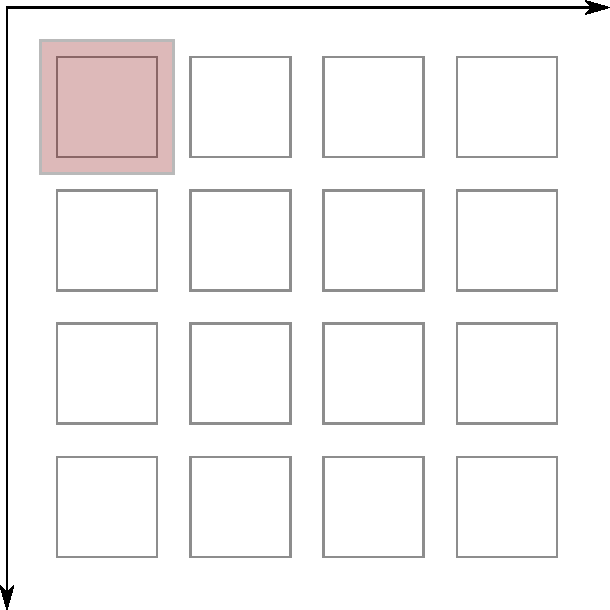
\includegraphics{figures/FullGridGeneral1}}}
	\subfigure[Schicht Level 1]{\resizebox{36mm}{!}{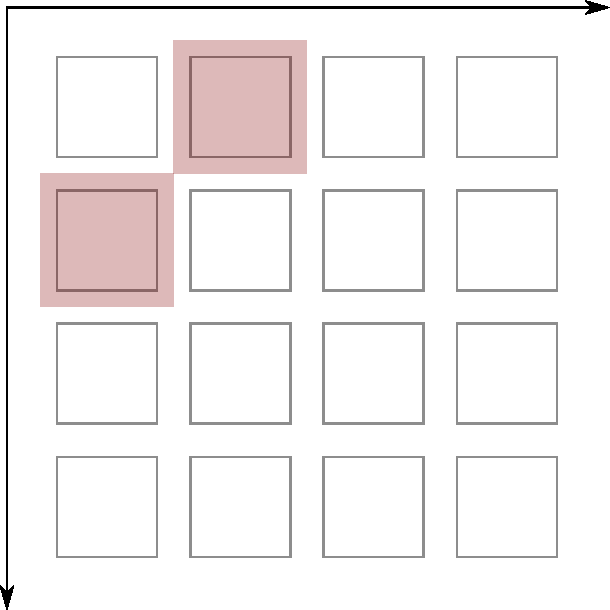
\includegraphics{figures/SparseGridGeneral2}}}
	\subfigure[Schicht Level 2]{\resizebox{36mm}{!}{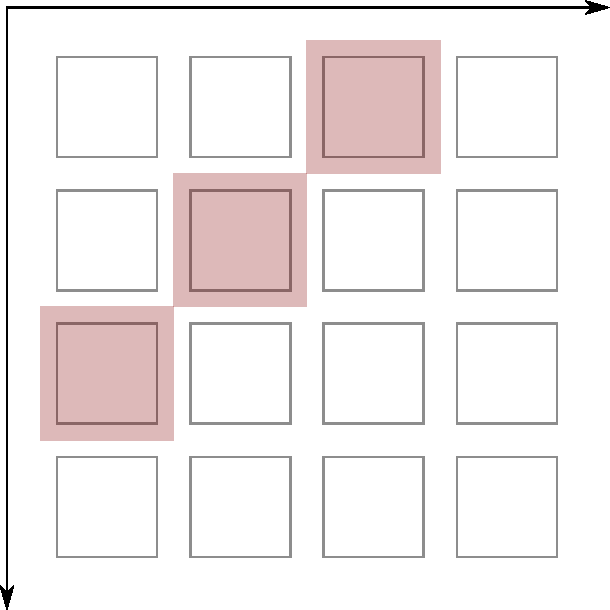
\includegraphics{figures/SparseGridGeneral3}}}
	\subfigure[Schicht Level 3]{\resizebox{36mm}{!}{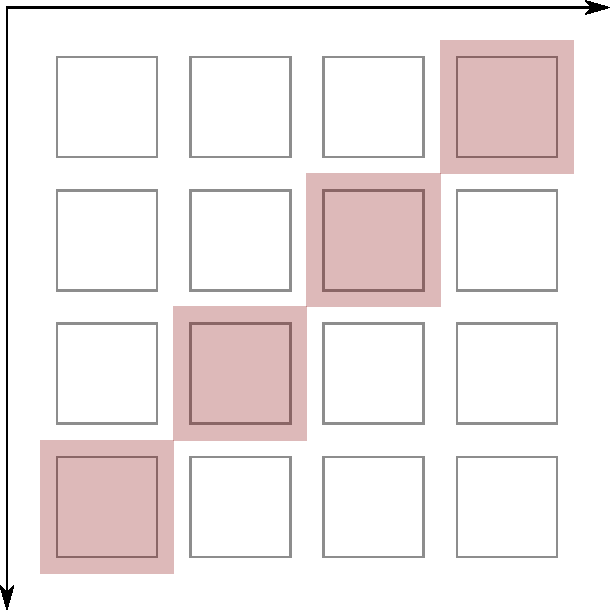
\includegraphics{figures/SparseGridGeneral4}}}
	\subfigure[Schicht Level 4]{\resizebox{36mm}{!}{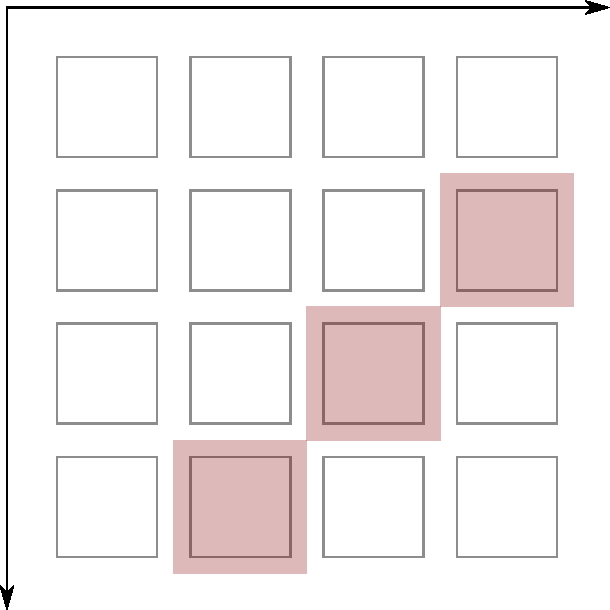
\includegraphics{figures/SparseGridGeneral5}}}
	\subfigure[Schicht Level 5]{\resizebox{36mm}{!}{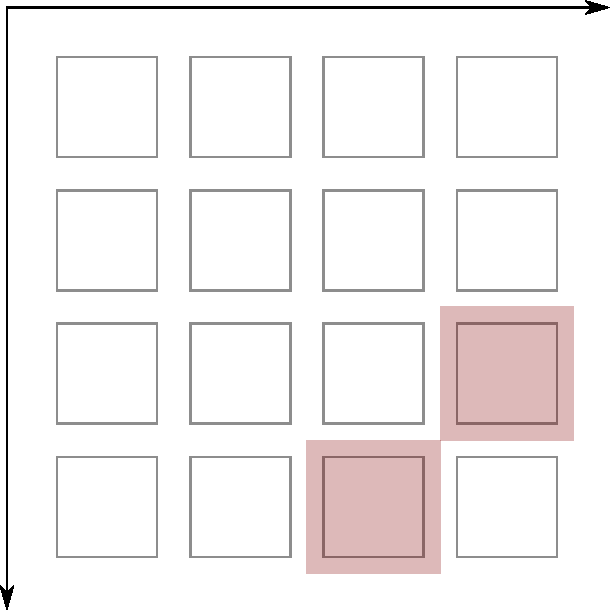
\includegraphics{figures/SparseGridGeneral6}}}
	\subfigure[Schicht Level 6]{\resizebox{36mm}{!}{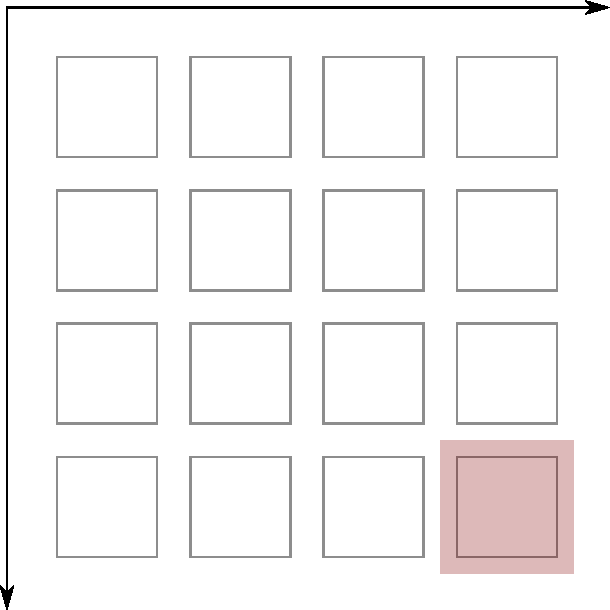
\includegraphics{figures/SparseGridGeneral7}}}
	\caption{Grobe Struktur bzgl. Inkremente dünne Gitter Strategie 2 Dimensionen}
	\label{fig:sparseGrid01}
\end{figure}

\subsubsection{Vorgehen}

Die auf Blöcke abgestimmte dünne Gitter Strategie arbeitet ebenfalls sehr einfach. Zunächst wird in MAX\_LEVEL\_SPARSE[] die maximale Anzahl der pro Gitterlevel neu hinzugekommen Punkte (in 2 Dimensionen also alle Punkte einer \underline{Diagonale!}) berechnet und gespeichert. Anschließend wird ein Zähler LEVEL\_SPARSE[] für jedes Gitterlevel eingerichtet der anfänglich auf 1 steht. Die Strategie iteriert dann über den Block und bestimmt für jeden Punkt die Gesamtsumme der Koordinatenlevel der Koordinaten. Daraus kann mit der Bedingung für dünne Gitter bestimmt werden zu welchem Gitterlevel der Punkt gehört. Für dieses Gitterlevel wird dem Punkt dann nur noch der passende Zähler zugewiesen und danach inkrementiert.

\subsubsection{Algorithmus in Pseudocode}

Dem Algorithmus wird eine Referenzkoordinate zum Block und ein Array, das jeder Zelle im Block die Nummer wann sie von der Strategie beschossen wird zuweist, übergeben.

\begin{tcolorbox}
	\begin{algorithmic}
		\Function{sparseGridStrat}{int[] blockShots, cell blockCoordinate}{:void}
		\State cell currentCell
		\State int shotNumber
		\For{int $i=0$; $i<$BlockSize; $i++$}
		\State \textsc{getCoordinateFromNumber}()
		\State int sumLevel $=0$
		\State sumLevel = \textsc{getSumLevel}()
		\State shotNumber = \textsc{calculateShotnumber}()
		\State blockShot[currentCell] = shotNumber
		\EndFor
		\EndFunction
	\end{algorithmic}
\end{tcolorbox}

\subsubsection{Erläuterung der Funktionen}
Die Funktion \textsc{getCoordinateFromNumber}() ist analog wie bei vollen Gittern.

Die Funktion \textsc{getSumLevel}() bestimmt in $O\left(d\cdot 2^{\lceil\log_2(N)\rceil}\right)$ die Summe der Koordinatenlevel von currentCell. Dabei werden alle $d$ Koordinaten der Zelle jeweils mit den $2^{\lceil\log_2(N)\rceil}$ Levelkoordinaten (vgl. Abbildung \ref{fig:redundancy}) verglichen, das Koordinatenlevel bestimmt und zur Summe sumLevel addiert.

Die Funktion \textsc{calculateShotnumber}() errechnet in $O(sumLevel) = O\left(d\cdot \lceil\log_2(N)\rceil\right)$ Schritten die Schussnummer von currentCell in dieser Strategie. Diese wird bestimmt durch Addition der MAX\_LEVEL\_SPARSE aller Gitterlevel bis sumLevel und LEVEL\_FULL[sumLevel]. Schließlich wird noch LEVEL\_FULL[sumLevel] inkrementiert.

\subsubsection{Komplexität}
Somit erhalten wir eine Laufzeitkomplexität von \\ $O\left(BlockSize\cdot d\left( 2^{\lceil\log_2(N)\rceil}+1+\lceil\log_2(N)\rceil\right)\right)$ für den dünnen Gitter Algorithmus. Die Speicherkomplexität beläuft sich dann auf $O(BlockSize)$. Bei $d$ Dimensionen kann BlockSize variiert werden zwischen $N^1$ und $N^d$. Wobei $N^d$ nur zu empfehlen ist wenn ausreichend Speicher zur Verfügung steht. 

%\subsection{Sobol Strategie}


\section{Ergebnisse}


Bestimmt man nun mithilfe der Implementation die Verteilungsfunktionen einer Stichprobe $\Omega_L \subseteq L_{all}$ von $\mathbf{T}^{\Omega_L}_{\strat}(\omega)$ und daraus dann $\mathbf{X}^{F_{all}}_{\strat}(\omega)$, können damit unterschiedliche Strategien auch über verschiedene Spielfeldgrößen gut miteinander verglichen werden.

\subsubsection{Random-Strategie}

Um bei der Random-Strategie brauchbare Ergebnisse zu erhalten werden mehrere Durchläufe (runs) ausgeführt und die Ergebnisse aller Durchläufe gemittelt.

TODO Ergebnisse kommentieren.

\begin{landscape}
	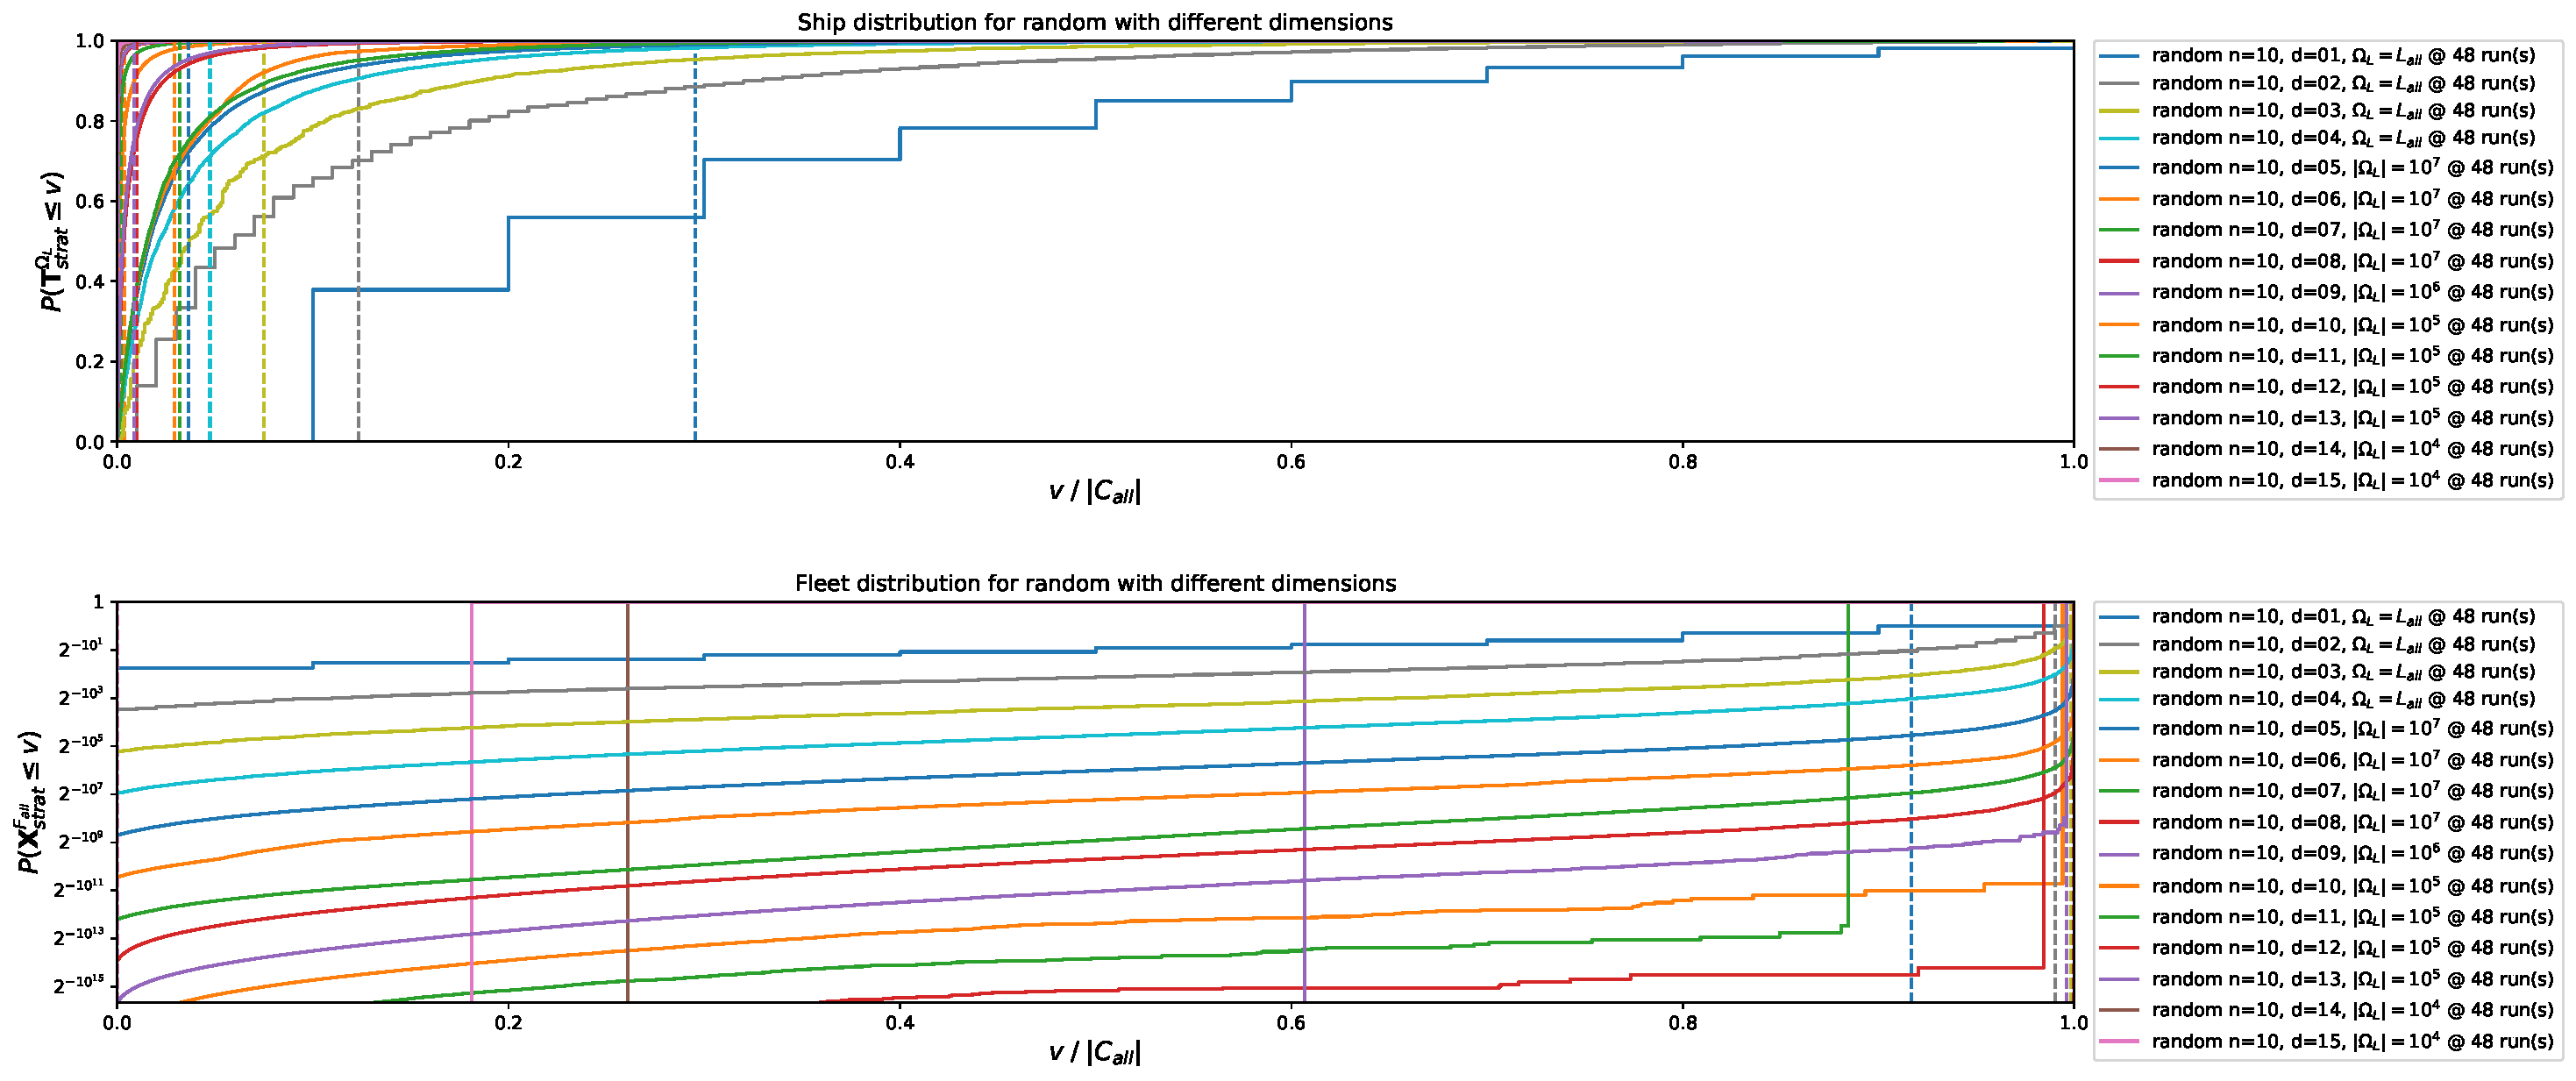
\includepdf[landscape=true]{figures/random_dimension.pdf}
\end{landscape}

\begin{landscape}
	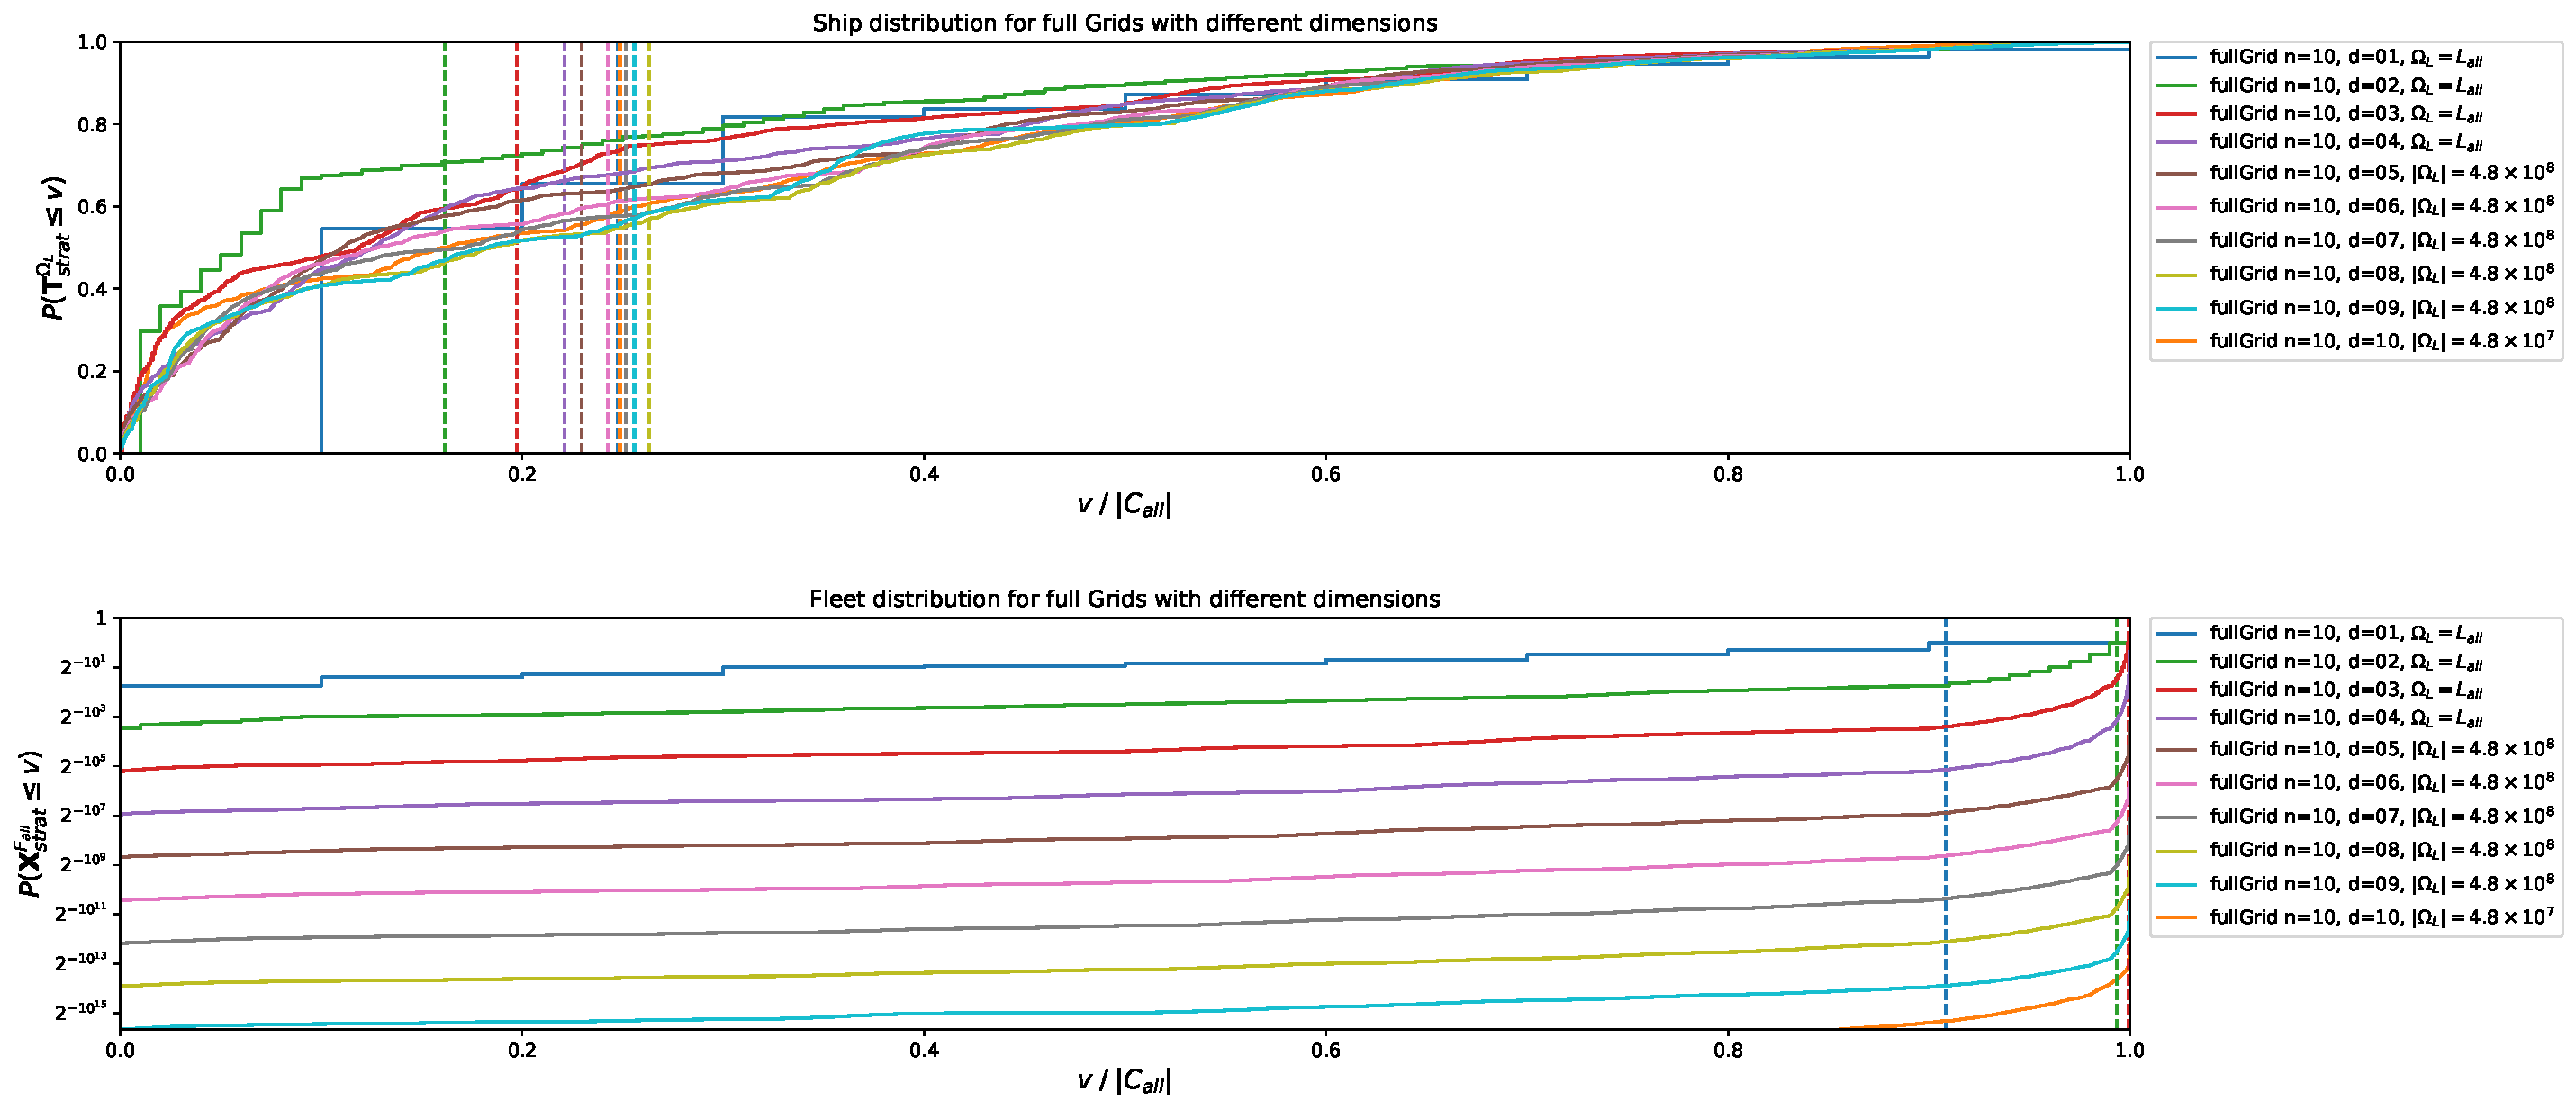
\includepdf[landscape=true]{figures/fullGrid_dimension.pdf}
\end{landscape}

\begin{landscape}
	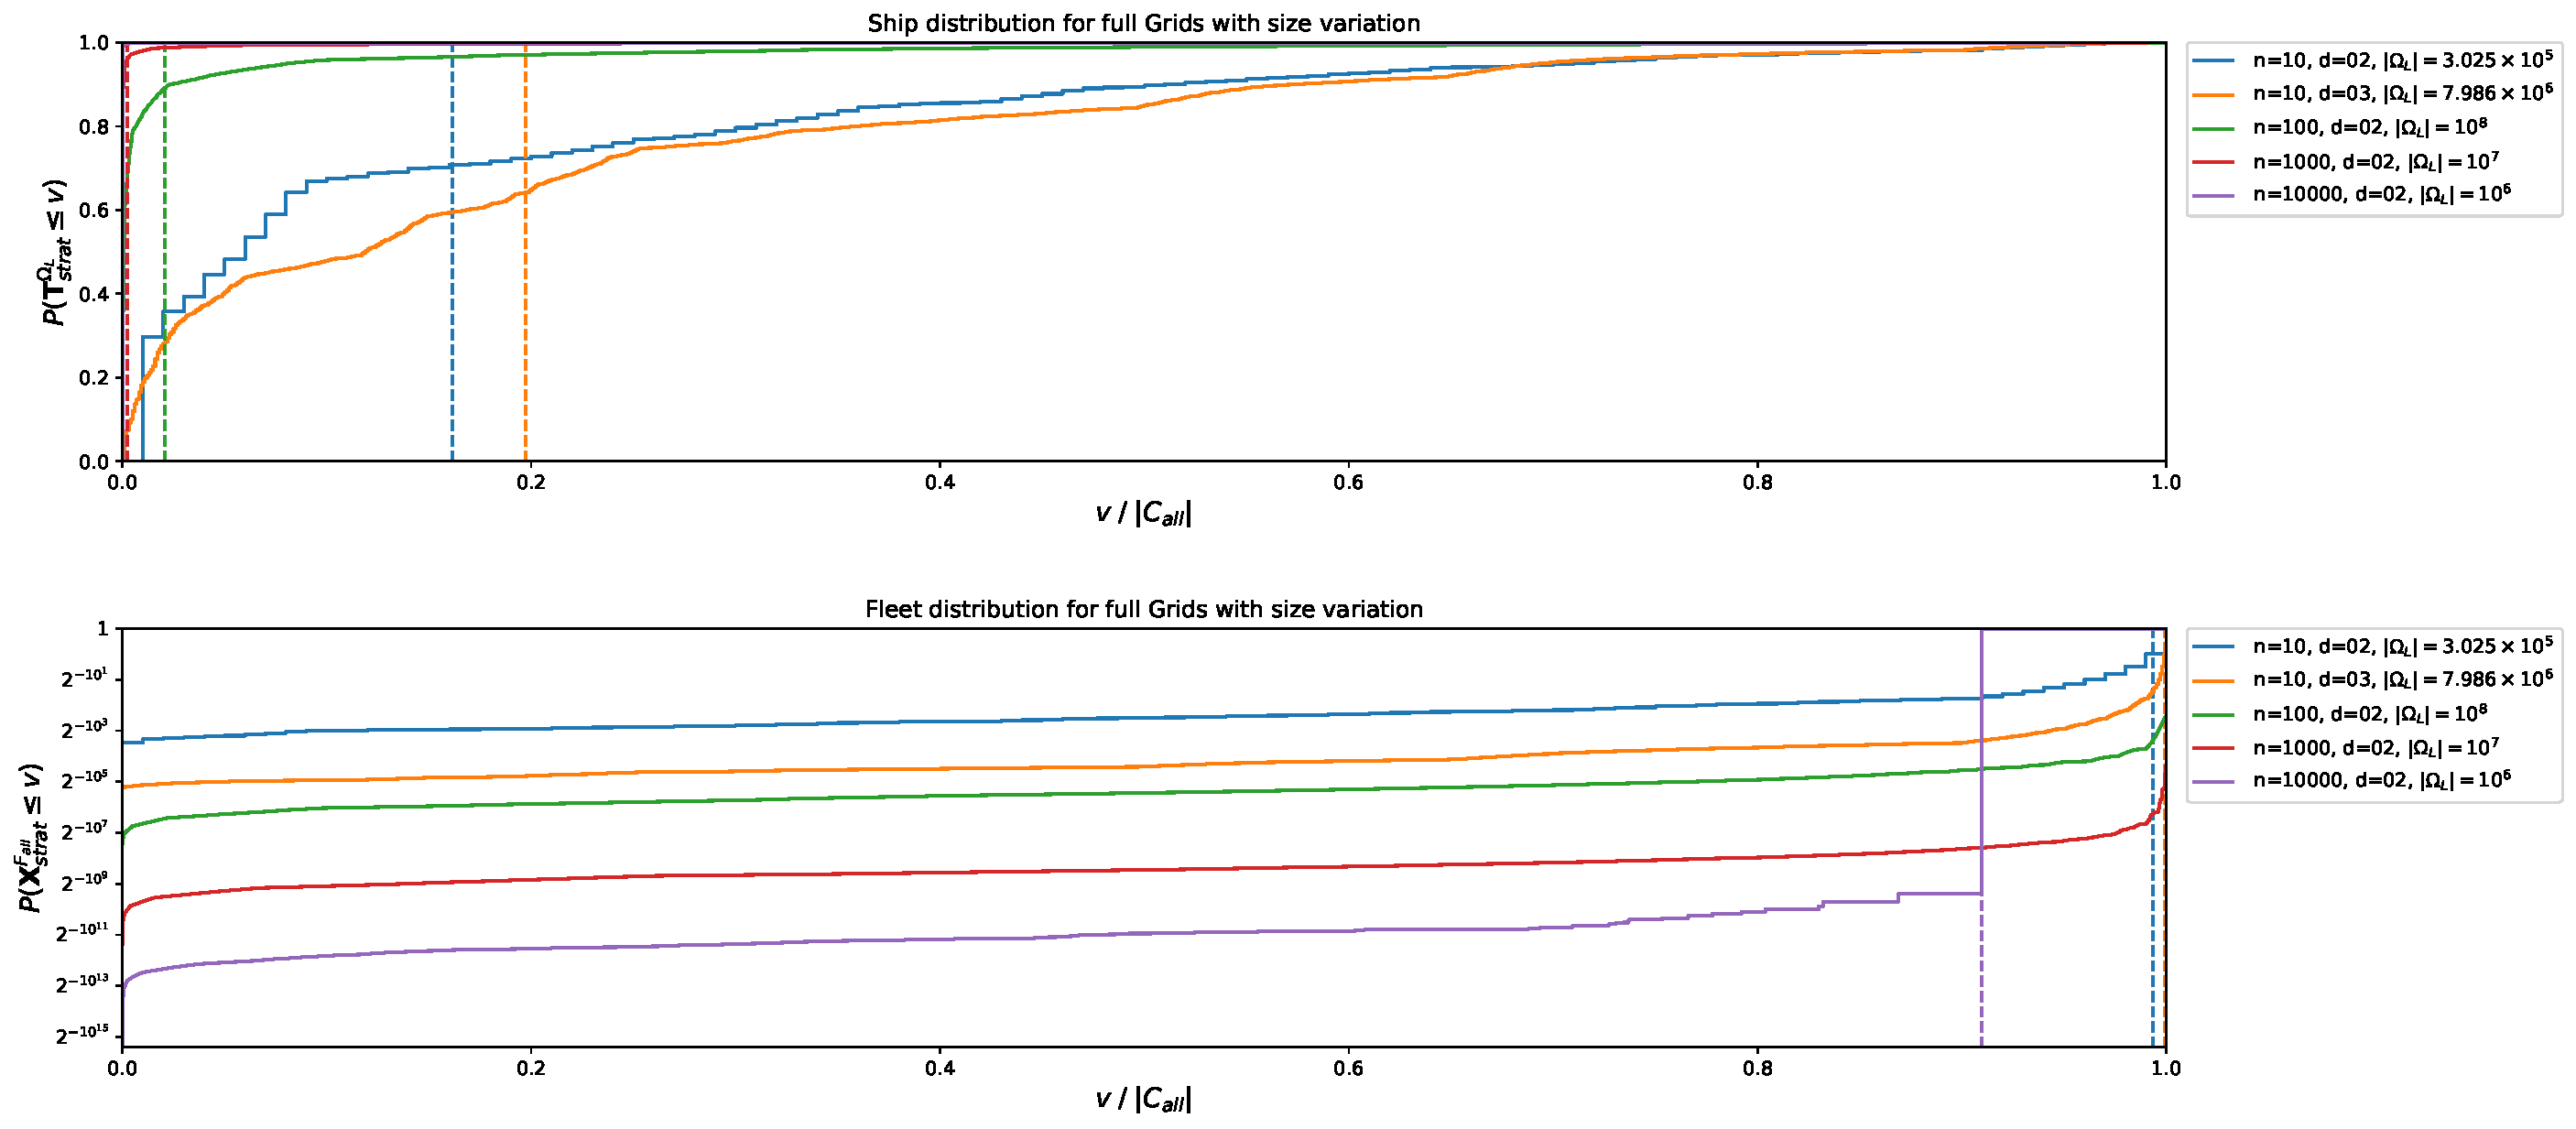
\includepdf[landscape=true]{figures/fullGrid_size.pdf}
\end{landscape}

\begin{landscape}
	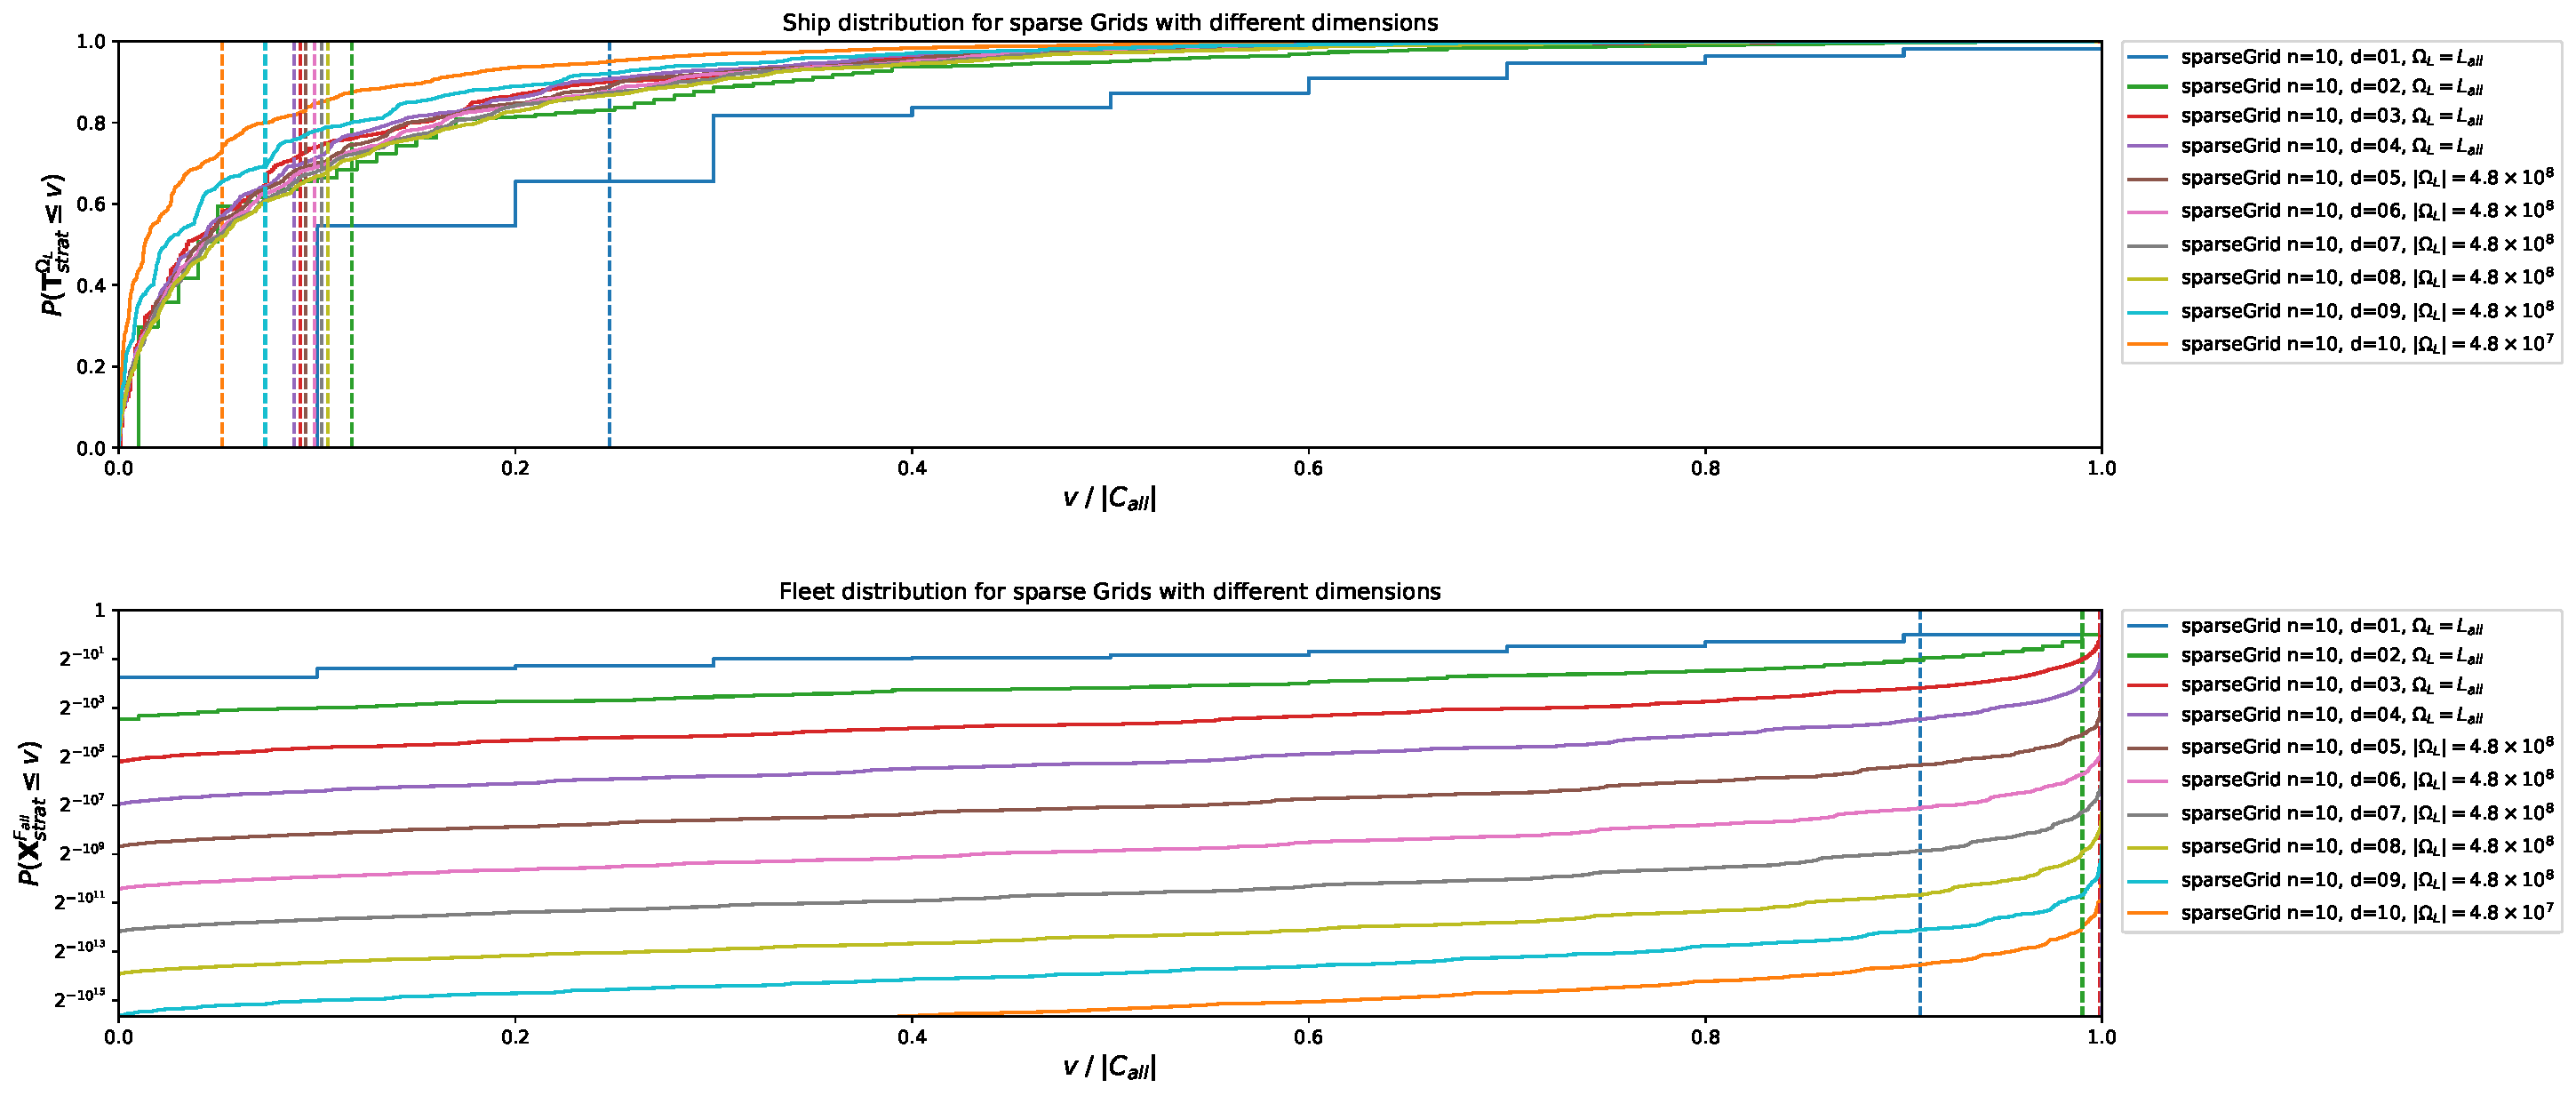
\includepdf[landscape=true]{figures/sparseGrid_dimension.pdf}
\end{landscape}

\begin{landscape}
	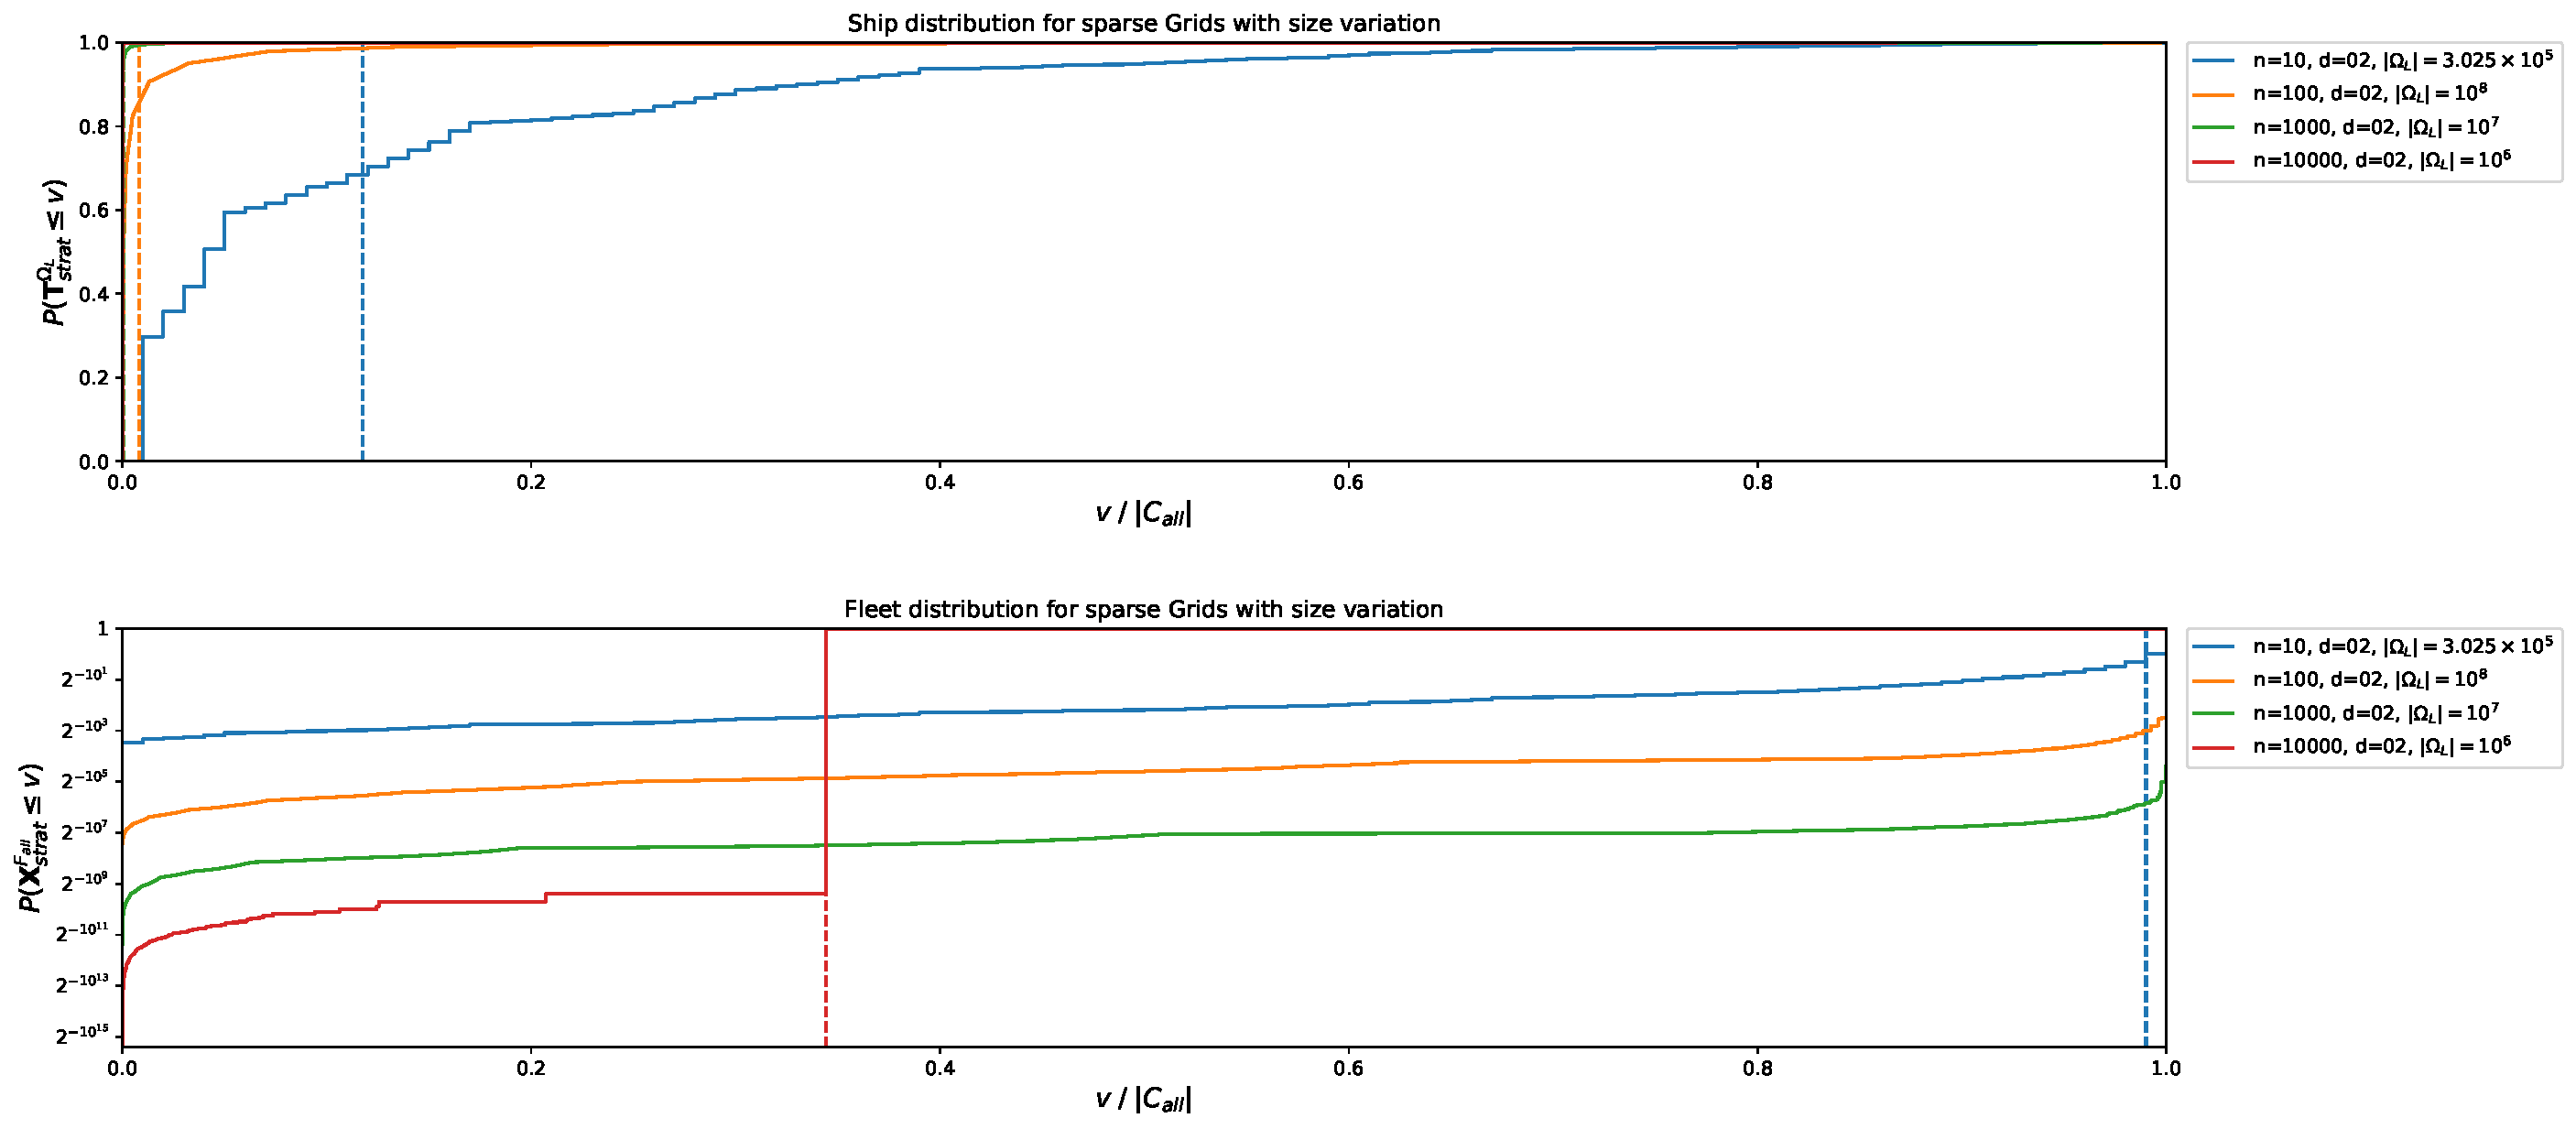
\includepdf[landscape=true]{figures/sparseGrid_size.pdf}
\end{landscape}

\begin{landscape}
	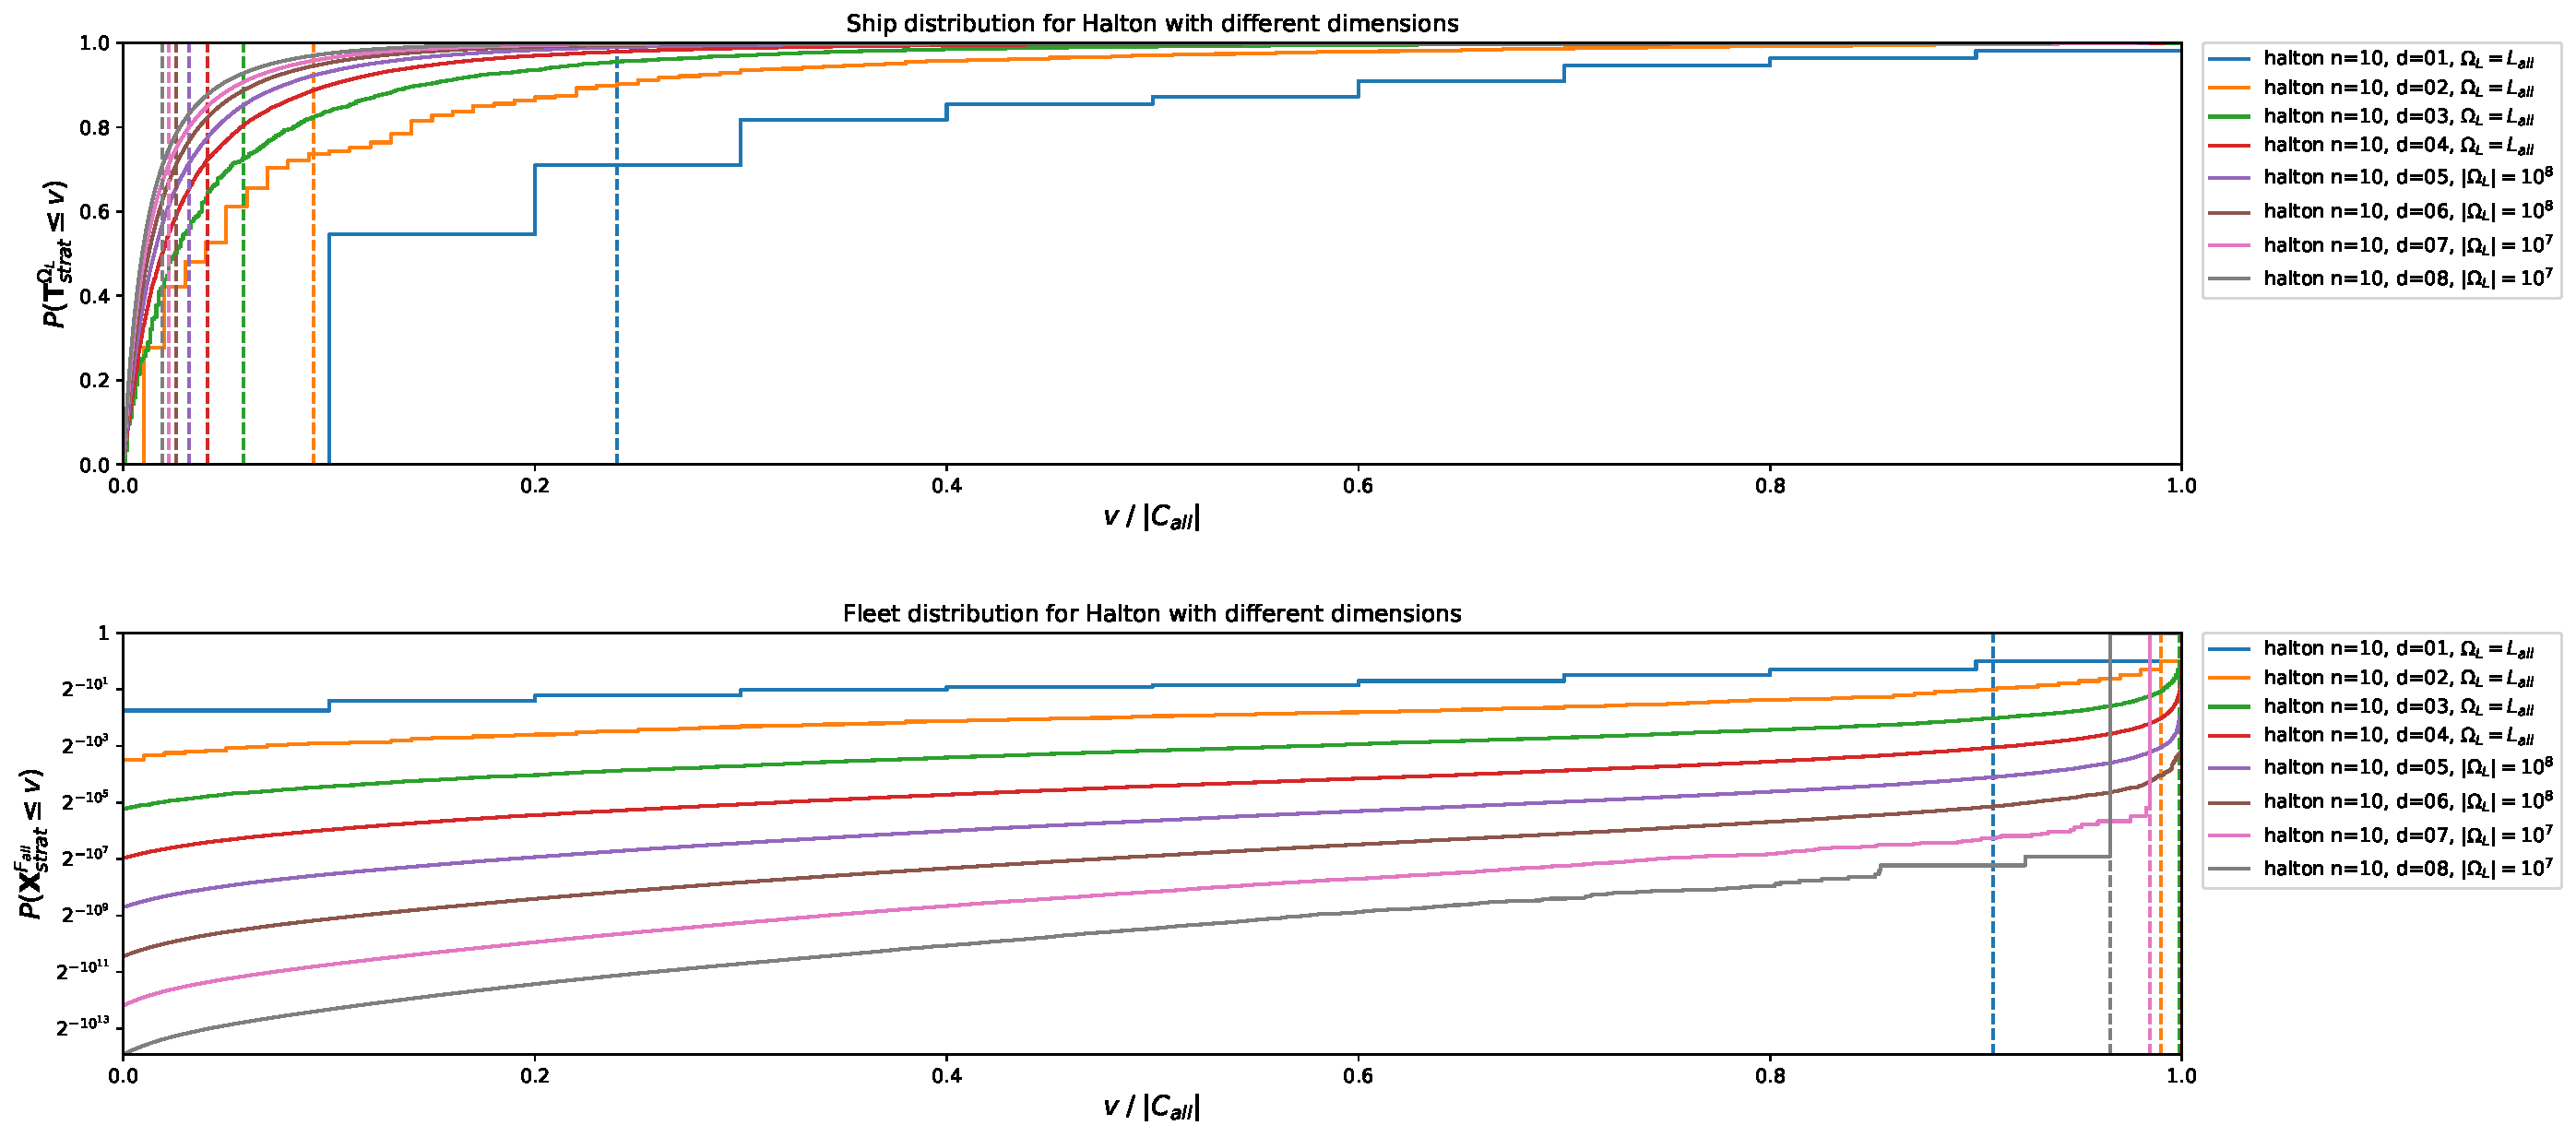
\includepdf[landscape=true]{figures/halton_dimension.pdf}
\end{landscape}

\begin{landscape}
	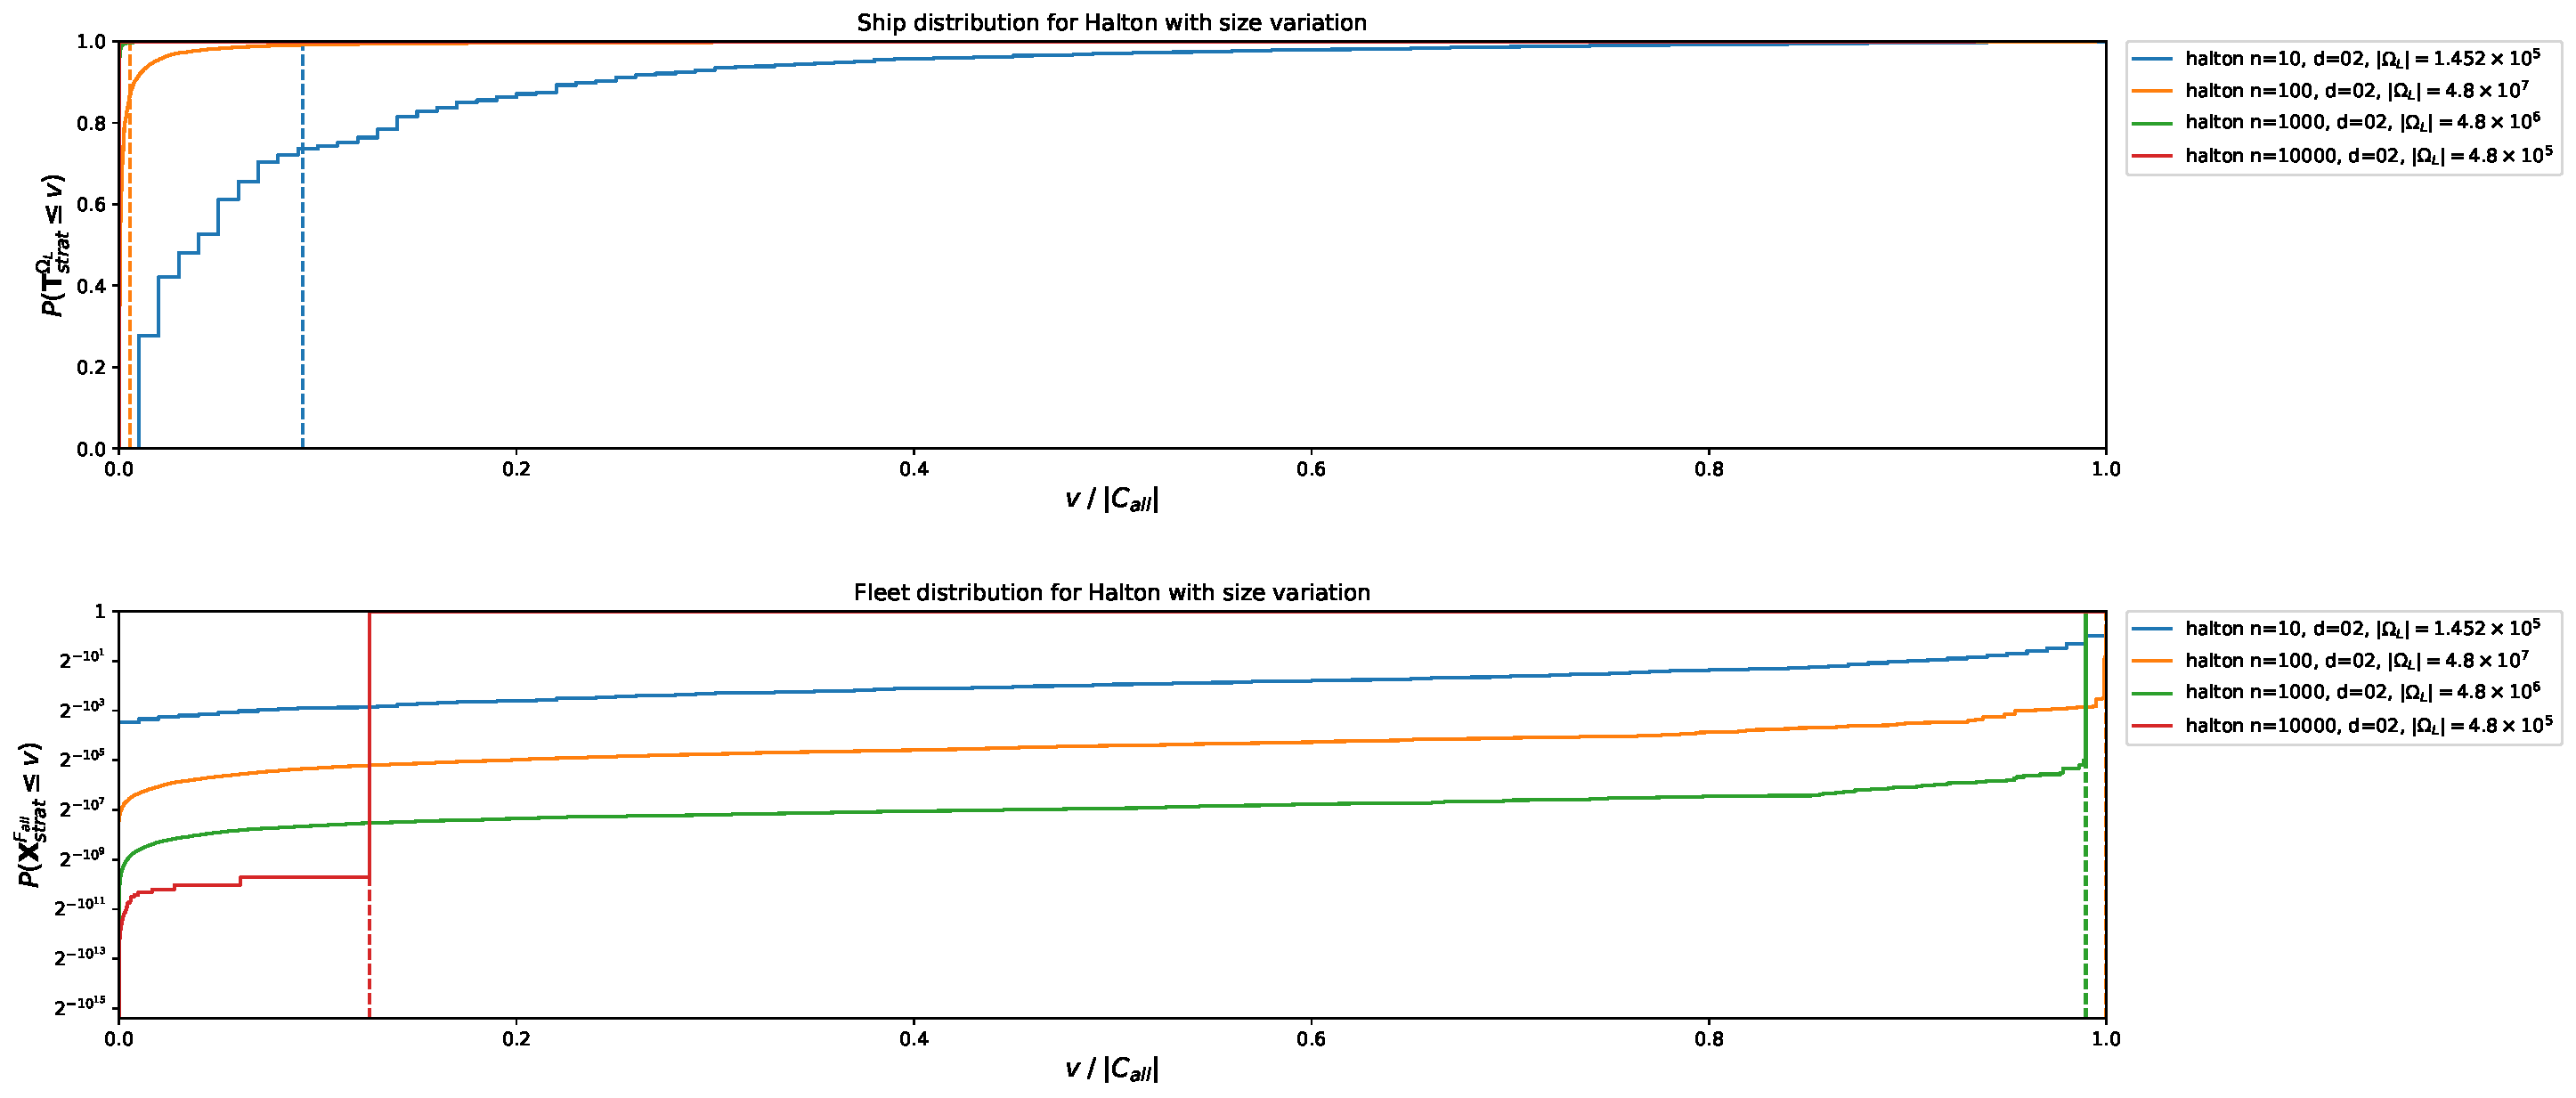
\includepdf[landscape=true]{figures/halton_size.pdf}
\end{landscape}

%\begin{landscape}
%	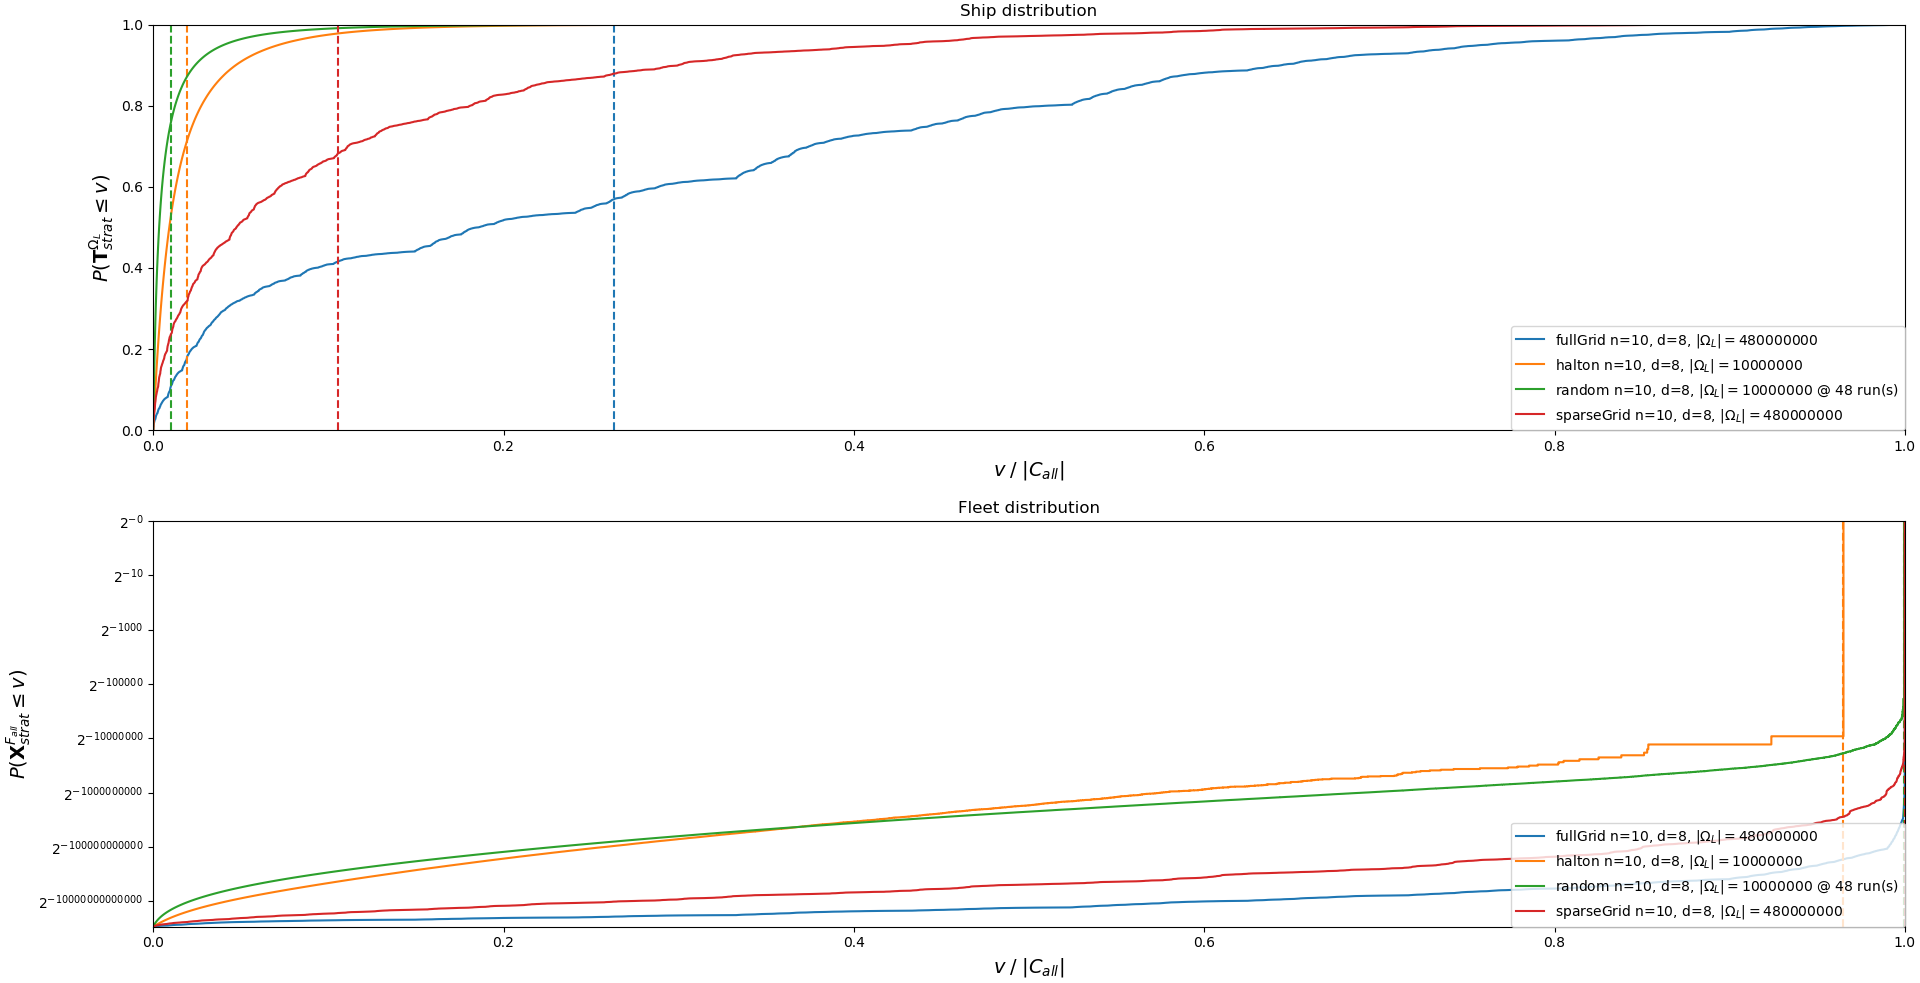
\includepdf[landscape=true]{figures/comparision.png}
%\end{landscape}


Wie bei dem betrachten des jeweils zweiten Plots, also den Ergebnissen für die Verteilungsfunktion von $\mathbf{X}^{F_{all}}_{\strat}$ auffällt, sind die Werte von $P(\mathbf{X}^{F_{all}}_{\strat} \leq v)$ sehr klein und streben erst sehr spät und ziemlich schnell gegen 1. Die Folge davon ist, dass der Erwartungswert $E(\mathbf{X}^{F_{all}}_{\strat})$ sehr groß ist. Genauer gesagt gilt $E(\mathbf{X}^{F_{all}}_{\strat}) \approx |C_{all}|$ selbst für kleine Spielfeldgrößen, wie z.B. $10^3$.

Dieses Phänomen ist Strategieunabhängig, d.h. die gewählte Strategie macht im Endeffekt keinen messbaren Unterschied darin, wie schnell eine zufällig gewählte Flotte versenkt werden kann. Selbst die bestmögliche Strategie würde im Vergleich zu einer sehr schlechten Strategie keinen messbaren Unterschied im Erwartungswert $E(\mathbf{X}^{F_{all}}_{\strat})$ zeigen.

\begin{satz}
Sei $\strat \in \strategies$ die verwendete Schuss-Strategie und $v \in \{1, \dots, |C_{all}|\}$
Sei außerdem $l=P(\mathbf{T}^{L_{all}}_{\strat} \leq v) |L_{all}|$

Dann gilt:
\begin{align}
\forall \strat \in \strategies \colon E(\mathbf{X}^{F_{all}}_{\strat}) \approx |C_{all}|
\nonumber
\end{align}

In anderen Worten, für jede Strategie ist die erwartet Anzahl an Schüssen, die benötigt werden um eine zufällig gewählte Flotte zu versenken ist circa so groß wie die Anzahl der Zellen, die das Spielfeld bestitzt.
\end{satz}

\begin{proof}
Sei $c_{last}=\strat(|C_{all}|)$ die letzte beschossene Zelle.
Sei $l_{last}=(c_{last}, c_{last})$ das Schiffe, das erst mit dem letzten Schuss versenkt wird.
Dann gibt es $F(L_{all} \setminus l_{last})=2^{|L_{all}|-1}$ viele Flotten, die $l_{last}$ nicht enthalten.
Daraus folgt aber, dass es ca. $\frac{1}{2} |F_{all}|$ viele Flotten gibt, die $l_{last}$ enthalten, und somit erst mit dem letzten möglichen Schuss versenkt werden.

Wendet man diese Argumentation jetzt iterativ an, d.h. man betrachtet danach die vorletzte beschossene Zelle, sieht man, dass es $(\frac{1}{2} + \frac{1}{4}) |F_{all}|$ viele Flotten gibt, die nach $|C_{all}| - 2$ vielen Schüssen noch nicht versenkt wurden.

Schon für kleine Werte wie z.B 10 gilt, dass es $(\frac{1}{2} + \frac{1}{4} + \dots + \frac{1}{2^{10}}) |F_{all}| \approx |F_{all}|$ viele Flotten gibt, die nach $|C_{all}| - 10$ vielen Schüssen noch nicht versenkt wurden.

Daraus folgt, dass für die erwartete Anzahl an Schüssen, um eine Flotte zu versenken gilt: $E(\mathbf{X}^{F_{all}}_{\strat}) \approx |C_{all}|$.
\qed
\end{proof}

Wie in einigen Graphen von $P(\mathbf{X}^{F_{all}}_{\strat} \leq v)$ vorallem für große Spielfelder außerdem zu sehen ist, gibt es Sprünge, in denen $P(\mathbf{X}^{F_{all}}_{\strat} \leq v)$ sofot den Wert 1 annimt. Diese sind die Folge von Messfehlern aufgrund verhältnismäßig kleiner Stichprobengrößen an Schiffen $|\Omega_L|$, die die Werte von $P(\mathbf{T}^{\Omega_L}_{\strat} \leq v)$ verfälschen und somit auch die daraus berechneten Werte von $P(\mathbf{X}^{F_{all}}_{\strat} \leq v)$ betreffen.

Um Strategien dennoch zu vergleichen und zu bewerten, kann $E(\mathbf{T}^{\Omega_L}_{\strat})$, d.h. der Erwartungswert für Schiffe herangezogen werden.



% Literaturverzeichnis ------------------------------------------------
\newpage
\bibliographystyle{alphadinLinkLocal}
%\bibliography{literatur} 

\begin{thebibliography}{WB95}
	\providecommand{\url}[1]{\texttt{#1}}
	\expandafter\ifx\csname urlstyle\endcsname\relax
	\providecommand{\doi}[1]{doi: #1}\else
	\providecommand{\doi}{doi: \begingroup \urlstyle{rm}\Url}\fi
	
	\bibitem[WB95]{WB95}
	\textsc{Welch}, G. ; \textsc{Bishop}, G.:
	\newblock An Introduction to the Kalman Filter  / UNC-CH Computer Science.
	\newblock \,Version:\,1995.
	\newblock  \url{http://www.cs.unc.edu/~welch/media/pdf/kalman_intro.pdf}
	(95-041). --
	\newblock Technical Report. --
	\newblock Online--Ressource
	
	\bibitem[M13]{M13}
	\textsc{Mehlbeer}, F.:
	\newblock \textit{Hierarchische Methoden am Beispiel von Schiffe versenken},
	\newblock Bachelorarbeit Nr.25,
	\newblock Universität Stuttgart,
	\newblock 2013
	
	\bibitem[P10]{P10}
	\textsc{Pflüger}, D.:
	\newblock \textit{Spatially Adaptive Sparse Grids for High-Dimensional Problems},
	\newblock Dissertation,,
	\newblock Technische Universität München,
	\newblock 2010
	
	\bibitem[GG08]{GG08}
	\textsc{Gerstner}, T. ; \textsc{Griebel}, M.:
	\newblock \textit{Sparse Grids},
	\newblock From Encyclopedia of Quantitative Finance,
	\newblock Universität Bonn,
	\newblock 2008
	
\end{thebibliography}


%\iffalse
\end{document}
%\fi
